% ============================================================================
% Introduction to Machine Learning and Deep Learning
% Summer School on AI for Economics and Finance
% University of Torino, August 24, 2026
% Duration: 45--50 minutes
% ============================================================================

\documentclass[aspectratio=169,11pt]{beamer}

% ---------- Theme and colors ----------
\usecolortheme{dove}
\setbeamertemplate{navigation symbols}{}
\setbeamertemplate{footline}{%
  \hfill\usebeamerfont{page number in head/foot}%
  \usebeamercolor[fg]{normal text}%
  \insertframenumber\,/\,\inserttotalframenumber\kern1em\vskip4pt}
\setbeamerfont{frametitle}{size=\huge}

% ---------- Packages ----------
\usepackage[utf8]{inputenc}
\usepackage[T1]{fontenc}
\usepackage{amsmath,amssymb,amsfonts}
\usepackage{bm}
\usepackage{graphicx}
\usepackage{tikz}
\usetikzlibrary{shapes,arrows.meta,positioning,calc,fit,backgrounds,patterns,decorations.pathreplacing}
\usepackage{pgfplots}
\pgfplotsset{compat=1.18}
% --- readable-from-the-back defaults for every plot ---
\pgfplotsset{every axis/.append style={
    tick label style={font=\footnotesize},
    label style={font=\small},
    title style={font=\small},
    legend style={font=\footnotesize}}}
\usepackage{booktabs}
\usepackage{hyperref}
\usepackage{multicol}
\usepackage{xcolor}
\usepackage{algorithm}
\usepackage{algorithmic}

% ---------- Custom colors ----------
\definecolor{uzhblue}{rgb}{0,0,0.5}
\definecolor{uzhgreylight}{RGB}{236,238,241}
\definecolor{uzhgreydark}{RGB}{81,86,94}
\definecolor{harvardcrimson}{RGB}{153,0,0}
\definecolor{unil@blue}{RGB}{0,140,204}
\definecolor{unil@black}{RGB}{35,31,32}
\definecolor{darkgreen}{RGB}{0,100,0}
\definecolor{darkred}{RGB}{139,0,0}
\definecolor{softblue}{RGB}{70,130,180}
\definecolor{softorange}{RGB}{230,159,0}
\definecolor{softgreen}{RGB}{0,158,115}

% ---------- Set beamer colors ----------
\setbeamercolor{frametitle}{bg=uzhgreylight, fg=uzhblue}
\setbeamercolor{title}{fg=uzhblue}
\setbeamercolor{structure}{fg=uzhblue}
\setbeamercolor{block title}{bg=unil@blue, fg=white}
\setbeamercolor{block body}{bg=uzhgreylight}
\setbeamercolor{block title alerted}{bg=darkred,fg=white}
\setbeamercolor{block body alerted}{bg=red!5}
\setbeamercolor{block title example}{bg=darkgreen,fg=white}
\setbeamercolor{block body example}{bg=green!5}
\setbeamercolor{item}{fg=unil@black}
\setbeamercolor{normal text}{fg=unil@black}

% ---------- Emphasis and hyperlinks ----------
\newcommand{\emphc}[1]{\textcolor{harvardcrimson}{#1}}
\hypersetup{colorlinks,linkcolor=harvardcrimson,urlcolor=harvardcrimson}

% ---------- Math commands ----------
\newcommand{\x}{\bm{x}}
\newcommand{\w}{\bm{w}}
\newcommand{\bb}{\bm{b}}
\newcommand{\z}{\bm{z}}
\newcommand{\W}{\bm{W}}
\newcommand{\X}{\bm{X}}
\renewcommand{\a}{\bm{a}}
\newcommand{\R}{\mathbb{R}}
\newcommand{\E}[1]{\mathbb{E}\!\left[#1\right]}
\DeclareMathOperator*{\argmin}{arg\,min}
\DeclareMathOperator*{\argmax}{arg\,max}

% ---------- Title ----------
\title[Deep Learning -- Torino 2026]%
{Summer School on AI for Economics and Finance}
\subtitle{Introduction to Machine Learning and Deep Learning}
\author{Simon Scheidegger}
\institute[HEC Lausanne]{HEC, University of Lausanne}
\date{University of Torino\\August 24, 2026}

\begin{document}

% ============================================================================
% PART 1: SETTING THE STAGE
% ============================================================================

% --- Slide 1: Title ---
{\setbeamercolor{background canvas}{bg=uzhgreylight}
\begin{frame}
\titlepage
\end{frame}
}

% --- Slide 2: Day 1 Overview ---
\begin{frame}{Day 1 at a Glance}
\begin{center}
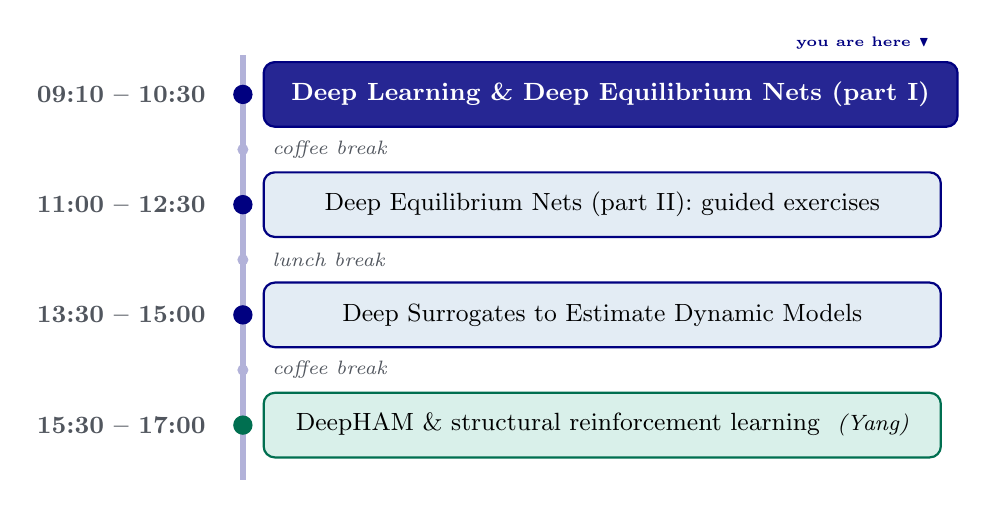
\begin{tikzpicture}[
    session/.style={rectangle, rounded corners=4pt, draw=uzhblue, thick, fill=softblue!15,
                    minimum width=8.6cm, minimum height=0.82cm, align=left, font=\small,
                    inner xsep=10pt, anchor=west},
    now/.style={session, fill=uzhblue!85, draw=uzhblue, text=white, font=\small\bfseries},
    guest/.style={session, fill=softgreen!15, draw=softgreen!70!black},
    pause/.style={font=\scriptsize\itshape, text=uzhgreydark, anchor=west},
    time/.style={font=\small\bfseries, text=uzhgreydark, anchor=east}
]
    % timeline spine
    \draw[uzhblue!30, line width=2pt] (0,0.5) -- (0,-4.9);

    % 09:10 current session
    \node[time] at (-0.35, 0) {09:10 -- 10:30};
    \node[now]  at (0.25, 0) {Deep Learning \& Deep Equilibrium Nets (part I)};
    \fill[uzhblue] (0,0) circle (3.5pt);
    \node[font=\tiny\bfseries, text=uzhblue, anchor=south east] at (8.85,0.45) {you are here $\blacktriangledown$};

    % coffee
    \node[pause] at (0.25,-0.7) {coffee break};
    \fill[uzhblue!30] (0,-0.7) circle (2pt);

    % 11:00 DEQN part II
    \node[time] at (-0.35,-1.4) {11:00 -- 12:30};
    \node[session] at (0.25,-1.4) {Deep Equilibrium Nets (part II): guided exercises};
    \fill[uzhblue] (0,-1.4) circle (3.5pt);

    % lunch
    \node[pause] at (0.25,-2.1) {lunch break};
    \fill[uzhblue!30] (0,-2.1) circle (2pt);

    % 13:30 surrogates
    \node[time] at (-0.35,-2.8) {13:30 -- 15:00};
    \node[session] at (0.25,-2.8) {Deep Surrogates to Estimate Dynamic Models};
    \fill[uzhblue] (0,-2.8) circle (3.5pt);

    % coffee
    \node[pause] at (0.25,-3.5) {coffee break};
    \fill[uzhblue!30] (0,-3.5) circle (2pt);

    % 15:30 Yang
    \node[time] at (-0.35,-4.2) {15:30 -- 17:00};
    \node[guest] at (0.25,-4.2) {DeepHAM \& structural reinforcement learning~~{\footnotesize\itshape (Yang)}};
    \fill[softgreen!70!black] (0,-4.2) circle (3.5pt);
\end{tikzpicture}
\end{center}

\vspace{0.1cm}
\begin{center}
{\footnotesize \textbf{Materials:}~\href{https://github.com/sischei/summer-school-AI-for-economics-and-finance-2026}{github.com/sischei/summer-school-AI-\ldots-2026}~~$\cdot$~~\textbf{Cloud:}~\href{https://nuvolos.cloud}{nuvolos.cloud}}
\end{center}
\end{frame}

% --- Slide 3: Roadmap ---
\begin{frame}{Roadmap of This Lecture (45--50 min)}
\begin{columns}[T]
\column{0.48\textwidth}
\textbf{Setting the Stage}~~\mbox{\small (6 min)}
\begin{itemize}
    \item Why deep learning, why now?
    \item Deep learning in economics and finance
\end{itemize}

\vspace{0.5em}
\textbf{Machine Learning Foundations}~~\mbox{\small (8 min)}
\begin{itemize}
    \item Supervised, unsupervised, RL
    \item The three-step ML recipe
\end{itemize}

\vspace{0.5em}
\textbf{From Perceptrons to Deep Nets}~~\mbox{\small (8 min)}
\begin{itemize}
    \item Neurons, activations, universal approximation
\end{itemize}

\column{0.48\textwidth}
\textbf{Training Neural Networks}~~\mbox{\small (12 min)}
\begin{itemize}
    \item Losses, (stochastic) gradient descent
    \item Backpropagation, optimizers
\end{itemize}

\vspace{0.5em}
\textbf{Generalization \& Regularization}~~\mbox{\small (6 min)}
\begin{itemize}
    \item Overfitting, early stopping, dropout
\end{itemize}

\vspace{0.5em}
\textbf{Outlook \& Practice}~~\mbox{\small (6 min)}
\begin{itemize}
    \item Beyond feedforward nets; software; exercises
\end{itemize}
\end{columns}
\end{frame}

% --- Slide 4: The Rise of Neural Networks ---
\begin{frame}{The Rise of Neural Networks}
\begin{center}
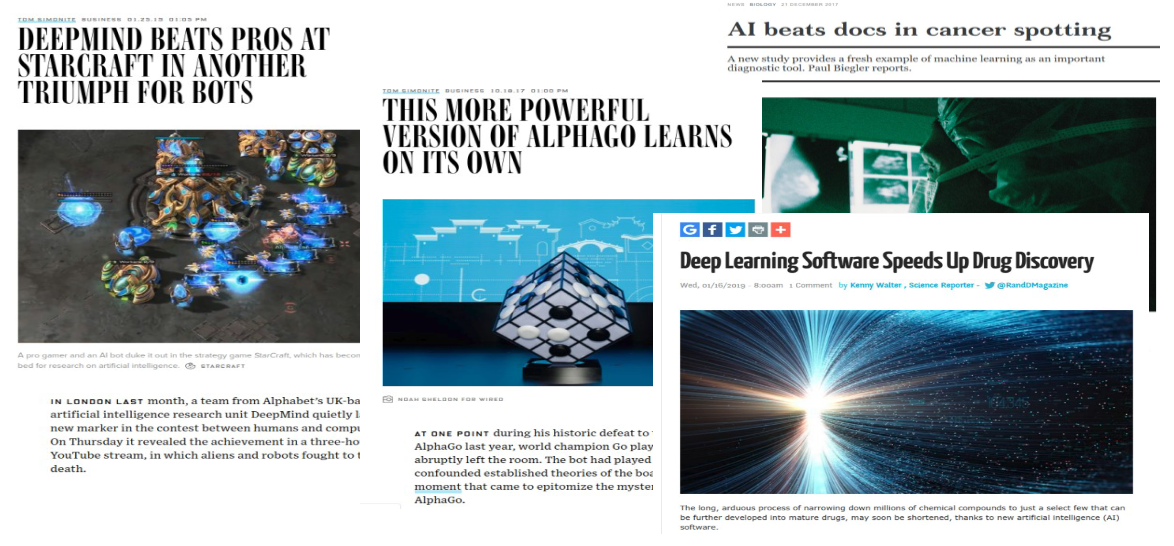
\includegraphics[width=\textwidth]{figures/rise.png}
\end{center}
\end{frame}

% --- Slide 5: AI Music Generation (Beethoven X) ---
\begin{frame}{AI Music Generation: Beethoven's Unfinished 10th}
\begin{columns}[T]
\column{0.36\textwidth}
\begin{center}

\includegraphics[width=0.92\textwidth]{figures/beethovenx_portrait.png}
\end{center}

\column{0.60\textwidth}
\textbf{Beethoven X, The AI Project:} musicologists, composers and AI researchers trained a network on Beethoven's complete works and sketches, then had it generate the \emphc{second and third movements} of his unfinished 10th symphony.

\vspace{0.3cm}
\begin{itemize}\itemsep3pt
    \item The network proposes continuations \emph{in Beethoven's style}; human experts curate and orchestrate.
    \item World premiere: Bonn, 9 October 2021.  Reception was mixed, which is itself a good prompt: \emph{what does the model actually learn?}
\end{itemize}

\vspace{0.3cm}
{\footnotesize Images and project: \emphc{Beethoven X, The AI Project}, \href{https://www.beethovenx-ai.com/}{beethovenx-ai.com}}
\end{columns}
\end{frame}

% --- Slide 6: Style Transfer ---
\begin{frame}{Neural Style Transfer}
\begin{center}
\begin{columns}[c]
\column{0.32\textwidth}
\begin{center}
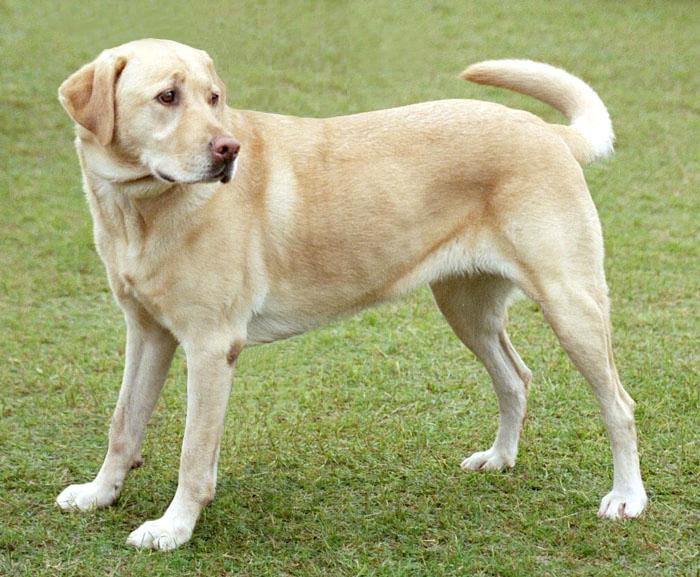
\includegraphics[width=\textwidth]{figures/dog1.png}\\[4pt]
{\small Content image}
\end{center}
\column{0.32\textwidth}
\begin{center}
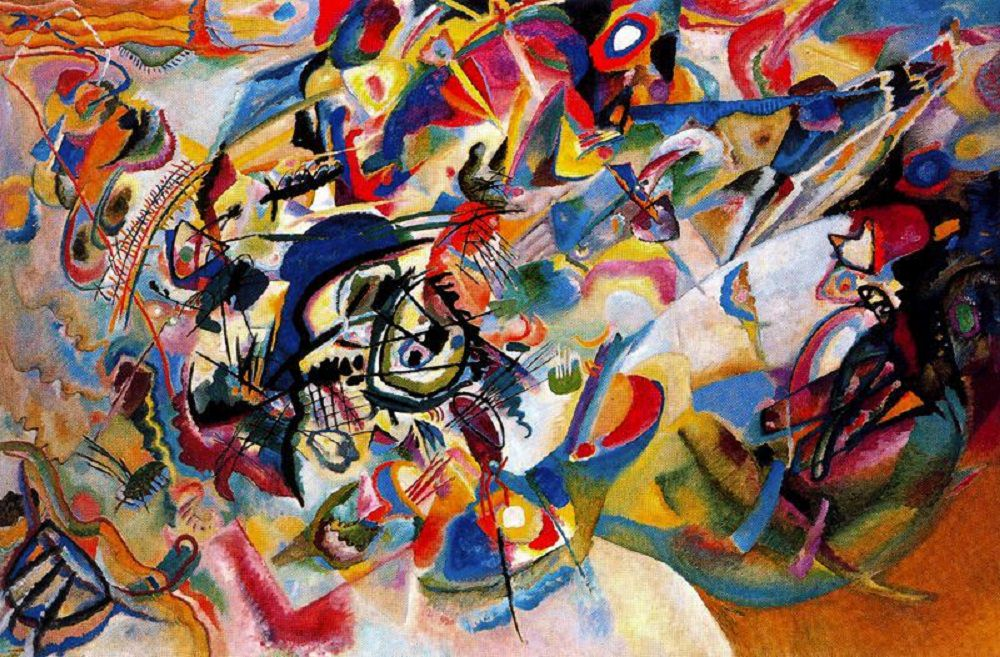
\includegraphics[width=\textwidth]{figures/kandinsky.png}\\[4pt]
{\small Style image (Kandinsky)}
\end{center}
\column{0.32\textwidth}
\begin{center}
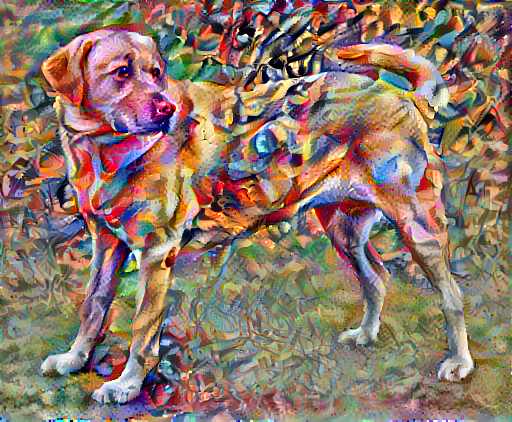
\includegraphics[width=\textwidth]{figures/dog2.png}\\[4pt]
{\small Result}
\end{center}
\end{columns}
\end{center}

\vspace{0.3cm}
{\small Gatys, Ecker \& Bethge (2015): a neural network separates and recombines content and style of images.}
\end{frame}

% --- Slide 7: Self-Driving Cars ---
\begin{frame}{Self-Driving Cars}
\begin{columns}[T]
\column{0.48\textwidth}
\begin{center}
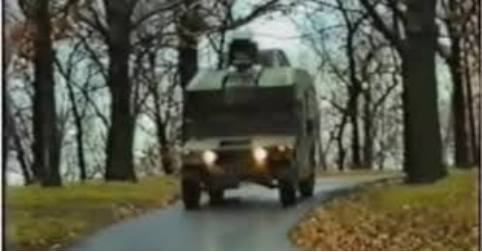
\includegraphics[width=\textwidth]{figures/alvinn.png}\\[4pt]
{\small \textbf{ALVINN} (1989), one of the first autonomous vehicles, using a simple neural network.}
\end{center}

\column{0.48\textwidth}
\begin{center}
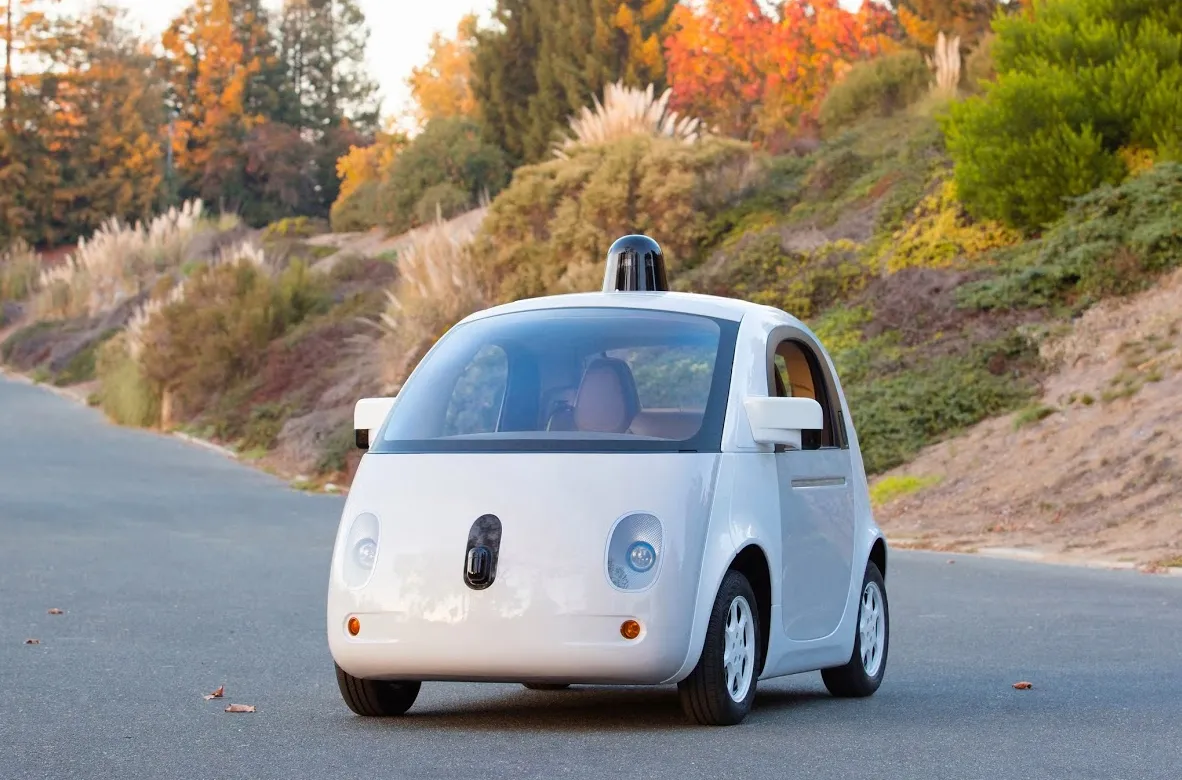
\includegraphics[width=\textwidth]{figures/waymo.png}\\[4pt]
{\small \textbf{Waymo} (2017+), deep learning for perception, prediction, and planning.}
\end{center}
\end{columns}
\end{frame}

% --- Slide 10: A Timeline of Deep Learning ---
\begin{frame}{A Timeline of Deep Learning}
\begin{center}
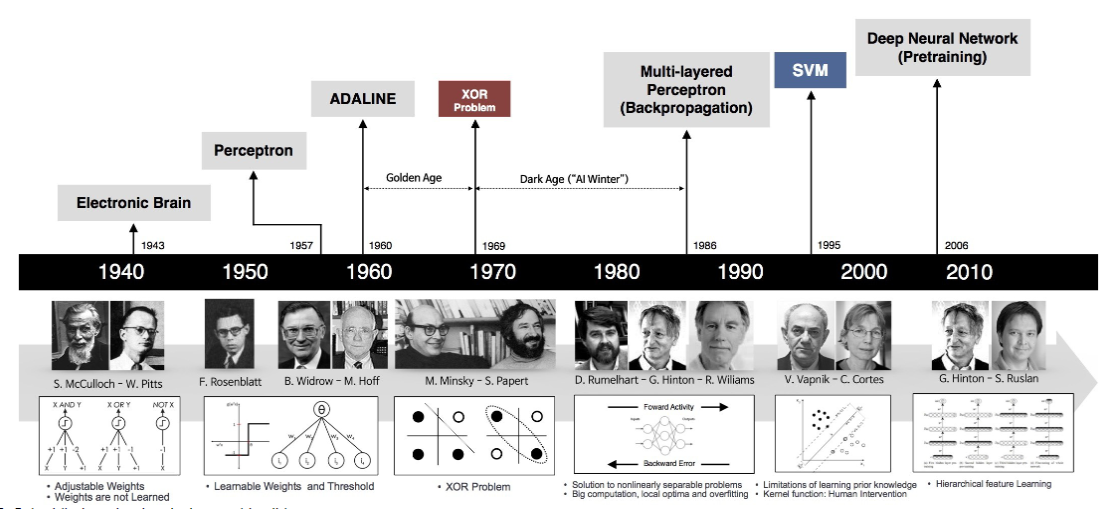
\includegraphics[width=\textwidth]{figures/timeline.png}
\end{center}
\end{frame}

% --- Slide 11: Deep Learning in Economics and Finance ---
\begin{frame}{Deep Learning in Economics and Finance}
\begin{columns}[T]
\column{0.48\textwidth}
\textbf{Forecasting \& nowcasting}
\begin{itemize}
    \item GDP nowcasting, inflation, yield curves
\end{itemize}

\vspace{0.45cm}
\textbf{Text \& communication}
\begin{itemize}
    \item Central-bank speeches, news sentiment, policy uncertainty
\end{itemize}

\column{0.48\textwidth}
\textbf{Financial stability \& supervision}
\begin{itemize}
    \item Fraud detection, credit risk, stress testing
\end{itemize}

\vspace{0.45cm}
\textbf{Structural models}
\begin{itemize}
    \item Solving and estimating DSGE, OLG and heterogeneous-agent models
\end{itemize}
\end{columns}

\vspace{0.7cm}
\begin{center}
\emphc{This summer school focuses on the last category:} deep learning as a \emph{computational} tool for economic modeling.
\end{center}
\end{frame}

% --- Slide 13: Why Deep Learning Now? ---
\begin{frame}{Why Deep Learning Now?}
Neural networks date back to the 1940s.  Three developments made them practical:

\vspace{0.4cm}
\begin{center}
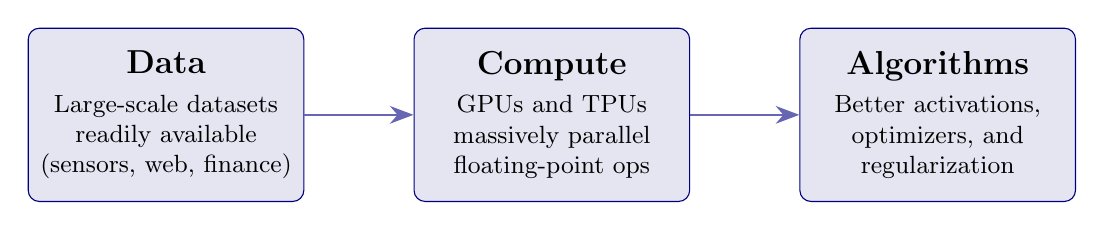
\begin{tikzpicture}[
    box/.style={rectangle, draw=uzhblue, fill=uzhblue!10, rounded corners=4pt,
                minimum width=3.5cm, minimum height=2.2cm, align=center, font=\small},
    arr/.style={-{Stealth[length=3mm]}, thick, uzhblue!60}
]
    \node[box] (data) at (0,0) {\textbf{\large Data}\\[3pt]Large-scale datasets\\readily available\\(sensors, web, finance)};
    \node[box] (hw) at (4.9,0) {\textbf{\large Compute}\\[3pt]GPUs and TPUs\\massively parallel\\floating-point ops};
    \node[box] (sw) at (9.8,0) {\textbf{\large Algorithms}\\[3pt]Better activations,\\optimizers, and\\regularization};

    \draw[arr] (data) -- (hw);
    \draw[arr] (hw) -- (sw);
\end{tikzpicture}
\end{center}

\vspace{0.3cm}
{\small Key milestones: Perceptron (1958), Backpropagation (1986), Convolutional nets (LeCun et al.\ 1989; LeNet-5, 1998), AlexNet (2012), Transformers (2017), ChatGPT (2022).}
\end{frame}


% ============================================================================
% PART 2: MACHINE LEARNING FOUNDATIONS
% ============================================================================

\section{Machine Learning Foundations}

% --- Section Divider ---
\begin{frame}{}
\begin{center}
{\Huge \textcolor{uzhblue}{Part I}}\\[0.8em]
{\LARGE Machine Learning Foundations}
\end{center}
\end{frame}

% --- Slide 14: What is Machine Learning? ---
\begin{frame}{What Is Machine Learning?}
\begin{columns}[T]
\column{0.45\textwidth}
\begin{center}
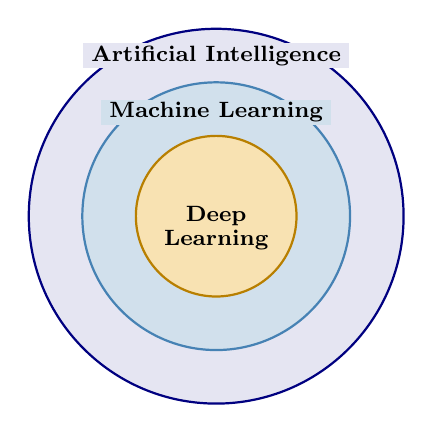
\begin{tikzpicture}[scale=0.85]
    % Concentric circles: AI > ML > DL
    \fill[uzhblue!10] (0,0) circle (2.8cm);
    \fill[softblue!25] (0,0) circle (2.0cm);
    \fill[softorange!30] (0,0) circle (1.2cm);
    \draw[uzhblue, thick] (0,0) circle (2.8cm);
    \draw[softblue, thick] (0,0) circle (2.0cm);
    \draw[softorange!80!black, thick] (0,0) circle (1.2cm);
    \node[font=\footnotesize\bfseries] at (0,0) {Deep};
    \node[font=\footnotesize\bfseries] at (0,-0.35) {Learning};
    \node[font=\footnotesize\bfseries, fill=softblue!25, inner xsep=3pt, inner ysep=1pt] at (0,1.55) {Machine Learning};
    \node[font=\footnotesize\bfseries, fill=uzhblue!10, inner xsep=3pt, inner ysep=1pt] at (0,2.4) {Artificial Intelligence};
\end{tikzpicture}
\end{center}

\column{0.52\textwidth}
\textbf{Classical programming:}

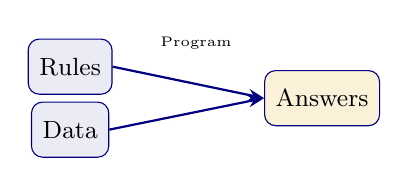
\begin{tikzpicture}[
    box/.style={rectangle, draw=uzhblue, fill=uzhblue!8, rounded corners,
                minimum height=7mm, font=\small, inner sep=4pt},
    arr/.style={-{Stealth[length=2mm]}, thick, uzhblue}]
    \node[box] (r) at (0,0) {Rules};
    \node[box] (d) at (0,-0.8) {Data};
    \node[box, fill=softorange!15] (a) at (3.2,-0.4) {Answers};
    \draw[arr] (r.east) -- (a.west);
    \draw[arr] (d.east) -- (a.west);
    \node[font=\tiny, above] at (1.6, 0.1) {Program};
\end{tikzpicture}

\vspace{0.4cm}
\textbf{Machine learning:}

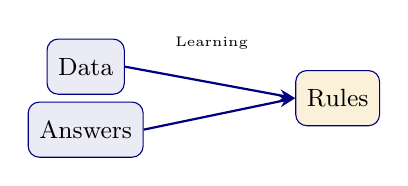
\begin{tikzpicture}[
    box/.style={rectangle, draw=uzhblue, fill=uzhblue!8, rounded corners,
                minimum height=7mm, font=\small, inner sep=4pt},
    arr/.style={-{Stealth[length=2mm]}, thick, uzhblue}]
    \node[box] (d) at (0,0) {Data};
    \node[box] (a) at (0,-0.8) {Answers};
    \node[box, fill=softorange!15] (r) at (3.2,-0.4) {Rules};
    \draw[arr] (d.east) -- (r.west);
    \draw[arr] (a.east) -- (r.west);
    \node[font=\tiny, above] at (1.6, 0.1) {Learning};
\end{tikzpicture}
\end{columns}
\end{frame}

% --- Slide 15: Types of ML ---
\begin{frame}{Types of Machine Learning}
\begin{columns}[T]
\column{0.32\textwidth}
\begin{block}{\centering Supervised}
    Given labeled pairs $\{(\x^{(i)}, y^{(i)})\}_{i=1}^{m}$, learn a mapping $h:\mathcal{X}\to\mathcal{Y}$.

    \vspace{0.3em}
    \textbf{Regression:} $y\in\R$\\
    \textbf{Classification:} $y\in\{1,\dots,K\}$
\end{block}

\column{0.32\textwidth}
\begin{block}{\centering Unsupervised}
    Given only $\{\x^{(i)}\}_{i=1}^{m}$, discover hidden structure.

    \vspace{0.3em}
    \textbf{Clustering:} group similar points\\
    \textbf{Dim.\ reduction:} compress features
\end{block}

\column{0.32\textwidth}
\begin{block}{\centering Reinforcement}
    An agent acts in an environment, receives rewards, and learns a policy $\pi$.

    \vspace{0.3em}
    \textbf{Policy:} $a_t = \pi(s_t)$\\
    \textbf{Goal:} maximize $\sum_t \gamma^t r_t$
\end{block}
\end{columns}

\vspace{0.5cm}
\begin{center}
{\small This morning we build up the \emph{supervised} pipeline (model, loss, optimizer),\\
then re-purpose it for the \emph{self-supervised} method at the heart of Day 1, \mbox{\textbf{Deep Equilibrium Nets}}.}
\end{center}
\end{frame}

% --- Slide 16: Supervised Regression ---
\begin{frame}{Supervised Learning: Regression}
\begin{columns}[T]
\column{0.52\textwidth}
\textbf{Goal:} predict a continuous target $y\in\R$ from features $\x\in\R^d$.

\vspace{0.3cm}
\textbf{Setup:}
\begin{itemize}
    \item Training data: $\{(\x^{(i)}, y^{(i)})\}_{i=1}^{m}$
    \item Model (hypothesis): $\hat{y} = h(\x;\bm{\theta})$
    \item Parameters $\bm{\theta}$ learned from data
\end{itemize}

\vspace{0.3cm}
\textbf{Linear example:}
\[
    h_{\bm{\theta}}(x) = \theta_0 + \theta_1 x
\]

\column{0.45\textwidth}
\begin{center}
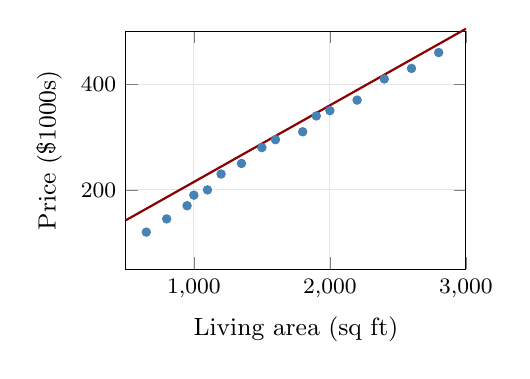
\begin{tikzpicture}
\begin{axis}[
    width=5.9cm, height=4.6cm,
    xlabel={Living area (sq ft)},
    ylabel={Price (\$1000s)},
    xmin=500, xmax=3000, ymin=50, ymax=500,
    grid=major, grid style={gray!20},
    clip=false
]
    % Scatter data
    \addplot[only marks, mark=*, mark size=1.5pt, softblue] coordinates {
        (650,120) (800,145) (950,170) (1000,190) (1100,200) (1200,230)
        (1350,250) (1500,280) (1600,295) (1800,310) (1900,340)
        (2000,350) (2200,370) (2400,410) (2600,430) (2800,460)
    };
    % Regression line
    \addplot[thick, darkred, domain=500:3000, samples=2]{70 + 0.145*x};
\end{axis}
\end{tikzpicture}
\end{center}
\end{columns}
\end{frame}

% --- Slide 17: Classification ---
\begin{frame}{Supervised Learning: Classification}
\begin{columns}[T]
\column{0.50\textwidth}
\textbf{Goal:} assign an input $\x$ to one of $K$ classes.

\vspace{0.3cm}
\textbf{Example, credit scoring:}
\begin{itemize}
    \item Features: income, savings
    \item Labels: low-risk / high-risk
    \item Decision boundary separates classes
\end{itemize}

\vspace{0.3cm}
A simple linear rule:
\[
    \text{if } \w^\top \x + b > 0 \;\Rightarrow\; \text{low-risk}
\]

\column{0.47\textwidth}
\begin{center}
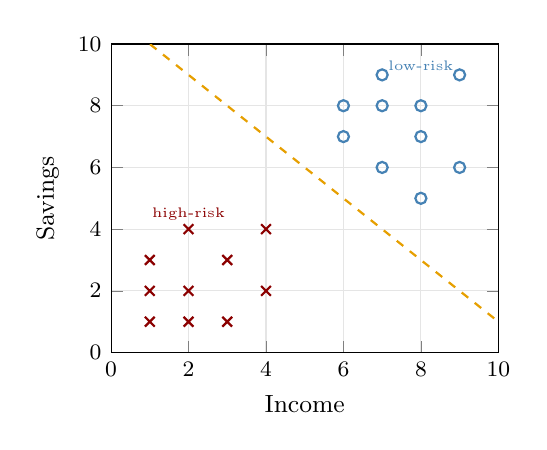
\begin{tikzpicture}
\begin{axis}[
    width=6.5cm, height=5.5cm,
    xlabel={Income}, ylabel={Savings},
    xmin=0, xmax=10, ymin=0, ymax=10,
    grid=major, grid style={gray!20},
]
    % Low-risk (blue)
    \addplot[only marks, mark=o, mark size=2pt, softblue, thick] coordinates {
        (6,7) (7,6) (8,5) (7,8) (8,7) (9,6) (6,8) (8,8) (9,9) (7,9)
    };
    % High-risk (red)
    \addplot[only marks, mark=x, mark size=2.5pt, darkred, thick] coordinates {
        (1,2) (2,1) (3,3) (2,4) (1,3) (4,2) (3,1) (2,2) (4,4) (1,1)
    };
    % Decision boundary
    \addplot[thick, softorange, dashed, domain=0:10, samples=2]{11-x};
    \node[font=\tiny, softblue] at (axis cs:8,9.3) {low-risk};
    \node[font=\tiny, darkred] at (axis cs:2,4.5) {high-risk};
\end{axis}
\end{tikzpicture}
\end{center}
\end{columns}
\end{frame}

% --- Slide 18: The ML Recipe ---
\begin{frame}{The Machine Learning Recipe}
Every machine learning algorithm follows the same three steps:

\vspace{0.5cm}
\begin{center}
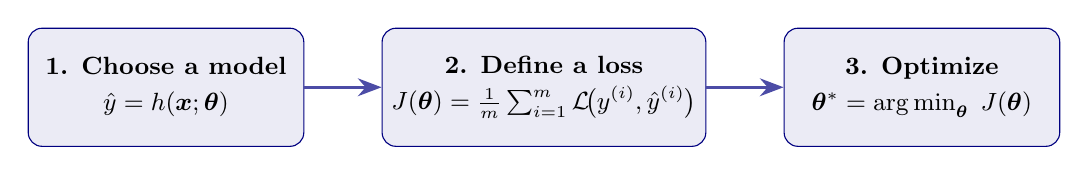
\begin{tikzpicture}[
    mlstep/.style={rectangle, draw=uzhblue, fill=uzhblue!8, rounded corners=5pt,
                 minimum width=3.5cm, minimum height=1.5cm, align=center, font=\small},
    arr/.style={-{Stealth[length=3mm]}, very thick, uzhblue!70}
]
    \node[mlstep] (m) at (0,0) {\textbf{1. Choose a model}\\[2pt]$\hat{y} = h(\x;\bm{\theta})$};
    \node[mlstep] (l) at (4.8,0) {\textbf{2. Define a loss}\\[2pt]$J(\bm{\theta}) = \frac{1}{m}\sum_{i=1}^{m}\mathcal{L}\!\big(y^{(i)},\hat{y}^{(i)}\big)$};
    \node[mlstep] (o) at (9.6,0) {\textbf{3. Optimize}\\[2pt]$\bm{\theta}^{*} = \argmin_{\bm{\theta}}\; J(\bm{\theta})$};

    \draw[arr] (m) -- (l);
    \draw[arr] (l) -- (o);
\end{tikzpicture}
\end{center}

\vspace{0.3cm}
\begin{block}{Cost function example (supervised regression: Mean Squared Error)}
\[
    J(\bm{\theta}) \;=\; \frac{1}{2m}\sum_{i=1}^{m}\!\big(h_{\bm{\theta}}(\x^{(i)}) - y^{(i)}\big)^{2}
\]
\end{block}
{\footnotesize\emphc{Same recipe, different loss.}  Deep Equilibrium Nets (next lecture) replace step~2 by an Euler-equation residual; steps~1 and~3 are unchanged.}
\end{frame}

% --- Slide 20: Unsupervised and Reinforcement Learning (brief) ---
\begin{frame}{Unsupervised and Reinforcement Learning (Brief)}
\begin{columns}[T]
\column{0.48\textwidth}
\textbf{Unsupervised learning:} no labels, only inputs $\{\x^{(i)}\}_{i=1}^{m}$; discover hidden structure.
\begin{itemize}
    \item \textbf{Clustering:} partition data into groups of similar points (customer segmentation).
    \item \textbf{Dimensionality reduction:} project to a lower-dimensional space (PCA, autoencoders).
\end{itemize}

\column{0.48\textwidth}
\textbf{Reinforcement learning:} an agent learns a policy $\pi(a\mid s)$ to maximize $\sum_{t}\gamma^t r_t$.

\vspace{0.2cm}
\begin{center}
\resizebox{0.95\linewidth}{!}{%
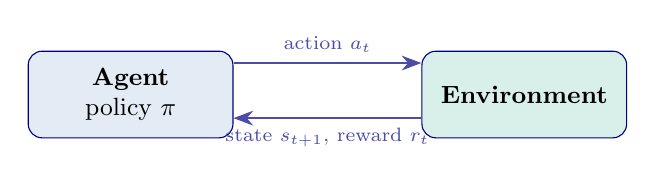
\begin{tikzpicture}[
    box/.style={rectangle, draw=uzhblue, fill=uzhblue!8, rounded corners=5pt,
                minimum width=2.6cm, minimum height=1.1cm, align=center, font=\small},
    arr/.style={-{Stealth[length=2.5mm]}, thick, uzhblue!70}
]
    \node[box, fill=softblue!15] (agent) at (0,0) {\textbf{Agent}\\policy $\pi$};
    \node[box, fill=softgreen!15] (env) at (5,0) {\textbf{Environment}};

    \draw[arr] ([yshift=4mm]agent.east) -- node[above, font=\scriptsize]{action $a_t$} ([yshift=4mm]env.west);
    \draw[arr] ([yshift=-3mm]env.west) -- node[below, font=\scriptsize]{state $s_{t+1}$, reward $r_t$} ([yshift=-3mm]agent.east);
\end{tikzpicture}}
\end{center}
\end{columns}

\vspace{0.5cm}
{\small Deep RL for heterogeneous-agent models is covered this afternoon (Yang, 15:30).  The neural network tools from this lecture are the building blocks for all of these paradigms.}
\end{frame}

% ============================================================================
% PART 3: FROM PERCEPTRONS TO DEEP NETWORKS
% ============================================================================

\section{Artificial Neural Networks}

% --- Section Divider ---
\begin{frame}{}
\begin{center}
{\Huge \textcolor{uzhblue}{Part II}}\\[0.8em]
{\LARGE From Perceptrons to Deep Networks}
\end{center}
\end{frame}

% --- Slide 21: Biological Neurons ---
\begin{frame}{Biological Neurons}
\begin{columns}[T]
\column{0.55\textwidth}
\begin{center}
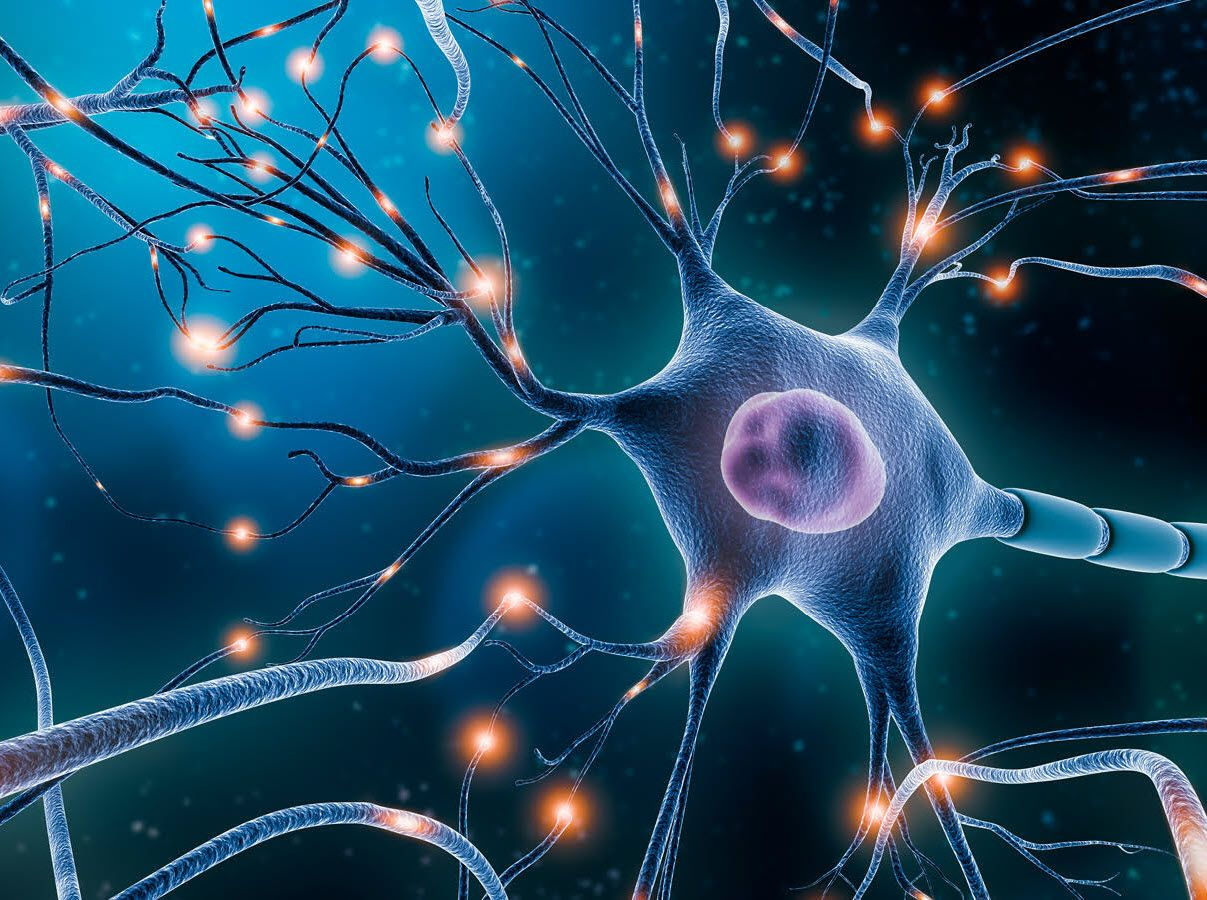
\includegraphics[width=\textwidth]{figures/neurons.png}
\end{center}

\column{0.42\textwidth}
\textbf{The brain} is a massively parallel computer made of $\sim$86 billion neurons.

\vspace{0.3cm}
Each neuron:
\begin{itemize}
    \item Receives signals via \textbf{dendrites}
    \item Integrates signals in the \textbf{cell body}
    \item Transmits output along the \textbf{axon}
    \item Communicates at \textbf{synapses}
\end{itemize}

\vspace{0.2cm}
{\small Artificial neural networks are a \textit{very loose} abstraction of this architecture.}
\end{columns}
\end{frame}

% --- Slide 22: McCulloch-Pitts Neuron ---
\begin{frame}{The Artificial Neuron (McCulloch \& Pitts, 1943)}
{\small\emphc{From biology to math:} synapses become weights, dendrites become inputs, integration becomes a sum, firing becomes a nonlinear activation.}
\vspace{0.05cm}
\begin{columns}[T]
\column{0.55\textwidth}
\begin{center}
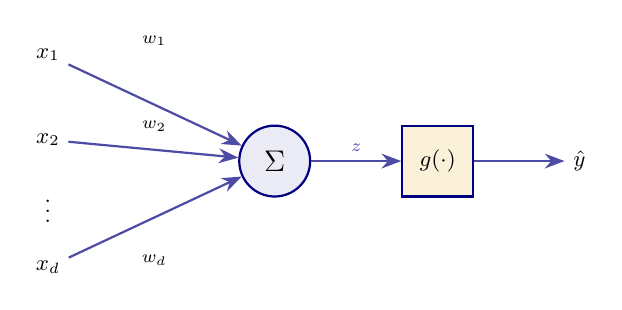
\begin{tikzpicture}[scale=0.9, transform shape,
    neuron/.style={circle, draw=uzhblue, thick, minimum size=10mm, fill=uzhblue!8},
    arr/.style={-{Stealth[length=2.5mm]}, thick, uzhblue!70}]

    % Inputs
    \node[font=\small] (x1) at (0,2) {$x_1$};
    \node[font=\small] (x2) at (0,0.8) {$x_2$};
    \node[font=\small] at (0,-0.1) {$\vdots$};
    \node[font=\small] (xm) at (0,-1) {$x_d$};

    % Weights
    \node[font=\scriptsize, above] at (1.5,2) {$w_1$};
    \node[font=\scriptsize, above] at (1.5,0.8) {$w_2$};
    \node[font=\scriptsize, below] at (1.5,-0.7) {$w_d$};

    % Sum node
    \node[neuron, font=\large] (sum) at (3.2,0.5) {$\Sigma$};

    % Activation
    \node[rectangle, draw=uzhblue, thick, fill=softorange!15,
          minimum width=10mm, minimum height=10mm, font=\small] (act) at (5.5,0.5) {$g(\cdot)$};

    % Output
    \node[font=\small] (out) at (7.5,0.5) {$\hat{y}$};

    % Arrows
    \draw[arr] (x1) -- (sum);
    \draw[arr] (x2) -- (sum);
    \draw[arr] (xm) -- (sum);
    \draw[arr] (sum) -- node[above, font=\scriptsize]{$z$} (act);
    \draw[arr] (act) -- (out);
\end{tikzpicture}
\end{center}

\column{0.42\textwidth}
{\small Three components:}
\begin{enumerate}\itemsep0pt\small
    \item \textbf{Weighted inputs} $w_i$ (synaptic weights)
    \item \textbf{Summation:} $z = \sum_{j=1}^{d} w_j x_j - \theta$ (threshold $\theta$)
    \item \textbf{Activation} $g(z)$: nonlinear function determining whether the neuron ``fires''
\end{enumerate}

\vspace{0.3cm}
{\footnotesize The 1943 model fired via a step function, and its weights were \emph{fixed}.  Making them \emphc{learnable} came later (Hebb 1949; Rosenblatt 1958).}
\end{columns}
\end{frame}

% --- Slide 24: The Perceptron ---
\begin{frame}{The Perceptron (Rosenblatt, 1958)}
\begin{columns}[T]
\column{0.48\textwidth}
\begin{center}
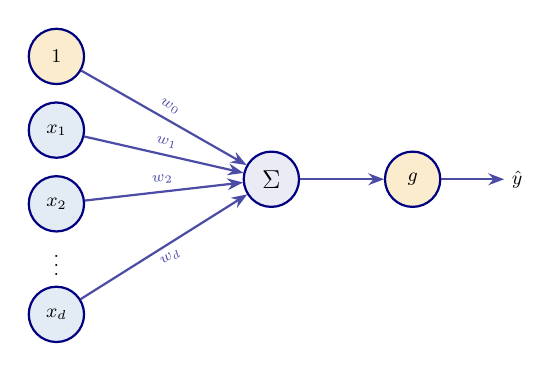
\begin{tikzpicture}[scale=0.78, transform shape,
    neuron/.style={circle, draw=uzhblue, thick, minimum size=9mm, fill=uzhblue!8},
    arr/.style={-{Stealth[length=2mm]}, thick, uzhblue!70}]

    % Bias
    \node[neuron, fill=softorange!20, font=\small] (b) at (0,3) {$1$};
    \node[neuron, fill=softblue!15, font=\small] (x1) at (0,1.8) {$x_1$};
    \node[neuron, fill=softblue!15, font=\small] (x2) at (0,0.6) {$x_2$};
    \node[font=\small] at (0,-0.3) {$\vdots$};
    \node[neuron, fill=softblue!15, font=\small] (xd) at (0,-1.2) {$x_d$};

    % Sum
    \node[neuron, font=\large] (sum) at (3.5,1) {$\Sigma$};

    % Activation
    \node[neuron, fill=softorange!20, font=\small] (act) at (5.8,1) {$g$};

    % Output
    \node[font=\small] (out) at (7.5,1) {$\hat{y}$};

    % Weight labels
    \draw[arr] (b) -- node[above, font=\scriptsize, sloped]{$w_0$} (sum);
    \draw[arr] (x1) -- node[above, font=\scriptsize, sloped]{$w_1$} (sum);
    \draw[arr] (x2) -- node[above, font=\scriptsize, sloped]{$w_2$} (sum);
    \draw[arr] (xd) -- node[below, font=\scriptsize, sloped]{$w_d$} (sum);
    \draw[arr] (sum) -- (act);
    \draw[arr] (act) -- (out);
\end{tikzpicture}
\end{center}

\column{0.48\textwidth}
\textbf{Forward pass:}
\[
    \hat{y} \;=\; g\!\left(w_0 + \sum_{j=1}^{d} x_j\, w_j\right) \;=\; g\!\big(\w^\top\x + b\big)
\]

\begin{itemize}\itemsep1pt
    \item {\small $b \equiv w_0$ is the \textbf{bias} (shifts the activation)}
    \item {\small $g(\cdot)$ is a nonlinear \textbf{activation function}}
\end{itemize}

\vspace{0.1cm}
{\footnotesize A weighted linear combination, then a nonlinearity.  \emphc{Without $g$ this is just linear regression.}}
\end{columns}

\vspace{0.15cm}
{\footnotesize \emphc{Minsky \& Papert (1969):} one perceptron cannot represent XOR, which is exactly why we need hidden layers.}
\end{frame}

% --- Slide 26: Activation Functions ---
\begin{frame}{Activation Functions}
\begin{center}
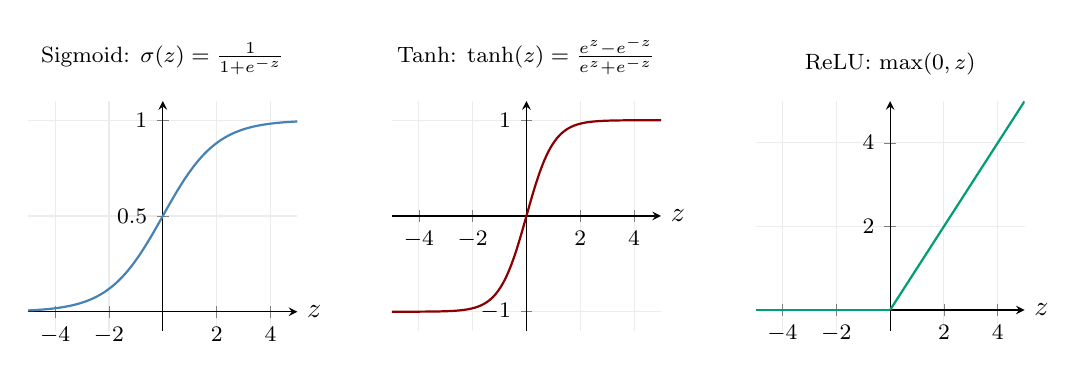
\begin{tikzpicture}
\begin{axis}[
    name=plot1,
    width=5cm, height=4.5cm,
    title={\footnotesize Sigmoid: $\sigma(z) = \frac{1}{1+e^{-z}}$},
    xlabel={$z$},    xmin=-5, xmax=5, ymin=-0.1, ymax=1.1,
    grid=major, grid style={gray!15},
    axis lines=middle,
    every axis x label/.style={at={(current axis.right of origin)}, anchor=west},
    every axis y label/.style={at={(current axis.above origin)}, anchor=south},
]
    \addplot[thick, softblue, domain=-5:5, samples=100]{1/(1+exp(-x))};
\end{axis}

\begin{axis}[
    at={($(plot1.east)+(1.2cm,0)$)}, anchor=west,
    name=plot2,
    width=5cm, height=4.5cm,
    title={\footnotesize Tanh: $\tanh(z) = \frac{e^z - e^{-z}}{e^z + e^{-z}}$},
    xlabel={$z$},    xmin=-5, xmax=5, ymin=-1.2, ymax=1.2,
    grid=major, grid style={gray!15},
    axis lines=middle,
    every axis x label/.style={at={(current axis.right of origin)}, anchor=west},
    every axis y label/.style={at={(current axis.above origin)}, anchor=south},
]
    \addplot[thick, darkred, domain=-5:5, samples=100]{tanh(x)};
\end{axis}

\begin{axis}[
    at={($(plot2.east)+(1.2cm,0)$)}, anchor=west,
    width=5cm, height=4.5cm,
    title={\footnotesize ReLU: $\max(0, z)$},
    xlabel={$z$},    xmin=-5, xmax=5, ymin=-0.5, ymax=5,
    grid=major, grid style={gray!15},
    axis lines=middle,
    every axis x label/.style={at={(current axis.right of origin)}, anchor=west},
    every axis y label/.style={at={(current axis.above origin)}, anchor=south},
]
    \addplot[thick, softgreen, domain=-5:0, samples=2]{0};
    \addplot[thick, softgreen, domain=0:5, samples=2]{x};
\end{axis}
\end{tikzpicture}
\end{center}

\vspace{-0.15cm}
\begin{center}
\begin{small}
\begin{tabular}{lcccc}
\toprule
& \textbf{Sigmoid} & \textbf{Tanh} & \textbf{ReLU} & \textbf{Swish} $z\sigma(z)$ / \textbf{Softplus} $\ln(1{+}e^z)$ \\
\midrule
Range & $(0,1)$ & $(-1,1)$ & $[0,\infty)$ & $\approx$ ReLU, but \emphc{smooth everywhere} \\
\bottomrule
\end{tabular}
\end{small}
\end{center}

\vspace{0.1cm}
{\footnotesize \emphc{Smoothness matters later:} ReLU has $g''=0$, so if the loss contains \emph{derivatives of the network} (Euler residuals, PDEs) use \textbf{tanh} or \textbf{Swish} instead.}
\end{frame}

% --- Slide 26b: Output activations as constraints ---
\begin{frame}{The Output Layer Is a Modeling Choice}
Hidden activations create flexibility.  The \emphc{output} activation encodes what you \emph{know} about the answer:

\vspace{0.2cm}
\begin{center}
\begin{small}
\renewcommand{\arraystretch}{1.25}
\begin{tabular}{lll}
\toprule
\textbf{Output head} & \textbf{Range} & \textbf{Use when} \\
\midrule
Identity (none)                & $\R$         & unconstrained regression \\
Softmax                        & simplex      & class probabilities \\
\textbf{Softplus} $\ln(1+e^z)$ & $(0,\infty)$ & must be positive (consumption) \\
\textbf{Sigmoid} $\sigma(z)$   & $(0,1)$      & a rate or share (savings rate) \\
\bottomrule
\end{tabular}
\end{small}
\end{center}

\vspace{0.2cm}
\begin{exampleblock}{Why this matters in the next lecture}
\small Constraints built into the \emph{architecture} hold \emphc{exactly} and cost nothing; a penalty in the loss holds only approximately.  Deep Equilibrium Nets use a sigmoid savings head so $C_t>0$ and $K_{t+1}>0$ \emph{before training starts}.
\end{exampleblock}
\end{frame}

% --- Slide 27: Why Nonlinearity? ---
\begin{frame}{Why Nonlinearity Matters}
\begin{columns}[T]
\column{0.47\textwidth}
\begin{center}
{\small\textbf{Linear activation} $\Rightarrow$ straight boundary}
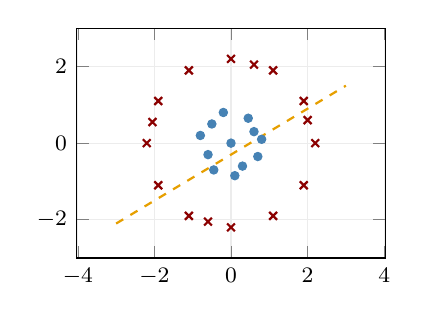
\begin{tikzpicture}
\begin{axis}[
    width=5.5cm, height=4.5cm,
    tick label style={font=\footnotesize},
    xmin=-3, xmax=3, ymin=-3, ymax=3,
    grid=major, grid style={gray!15},
    axis equal,
]
    \addplot[only marks, mark=*, mark size=1.5pt, softblue] coordinates {(0,0) (0.6,0.3) (-0.5,0.5) (0.3,-0.6) (-0.6,-0.3) (0.8,0.1) (-0.2,0.8) (0.1,-0.85) (-0.8,0.2) (0.45,0.65) (-0.45,-0.7) (0.7,-0.35)};
    \addplot[only marks, mark=x, mark size=2pt, darkred, thick] coordinates {(2.2,0) (1.9,1.1) (1.1,1.9) (0,2.2) (-1.1,1.9) (-1.9,1.1) (-2.2,0) (-1.9,-1.1) (-1.1,-1.9) (0,-2.2) (1.1,-1.9) (1.9,-1.1) (2.0,0.6) (0.6,2.05) (-2.05,0.55) (-0.6,-2.05)};
    % any straight line cuts both classes
    \addplot[thick, softorange, dashed, domain=-3:3, samples=2]{0.6*x-0.3};
\end{axis}
\end{tikzpicture}\\[2pt]
{\footnotesize\bfseries\color{softorange}no straight line can separate them}
\end{center}

\column{0.47\textwidth}
\begin{center}
{\small\textbf{Nonlinear activation} $\Rightarrow$ curved boundary}
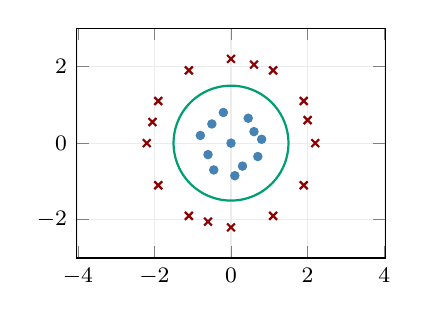
\begin{tikzpicture}
\begin{axis}[
    width=5.5cm, height=4.5cm,
    tick label style={font=\footnotesize},
    xmin=-3, xmax=3, ymin=-3, ymax=3,
    grid=major, grid style={gray!15},
    axis equal,
]
    \addplot[only marks, mark=*, mark size=1.5pt, softblue] coordinates {(0,0) (0.6,0.3) (-0.5,0.5) (0.3,-0.6) (-0.6,-0.3) (0.8,0.1) (-0.2,0.8) (0.1,-0.85) (-0.8,0.2) (0.45,0.65) (-0.45,-0.7) (0.7,-0.35)};
    \addplot[only marks, mark=x, mark size=2pt, darkred, thick] coordinates {(2.2,0) (1.9,1.1) (1.1,1.9) (0,2.2) (-1.1,1.9) (-1.9,1.1) (-2.2,0) (-1.9,-1.1) (-1.1,-1.9) (0,-2.2) (1.1,-1.9) (1.9,-1.1) (2.0,0.6) (0.6,2.05) (-2.05,0.55) (-0.6,-2.05)};
    % closed circular boundary separates the two rings exactly
    \addplot[thick, softgreen, domain=0:360, samples=120, smooth]
        ({1.5*cos(x)}, {1.5*sin(x)});
\end{axis}
\end{tikzpicture}\\[2pt]
{\footnotesize\bfseries\color{softgreen}a curved boundary separates them exactly}
\end{center}
\end{columns}

\vspace{0.15cm}
\begin{alertblock}{Mathematical reason}
\small A composition of linear maps is still linear: $\W_2(\W_1\x+\bb_1)+\bb_2 = \W_2\W_1\x + (\W_2\bb_1+\bb_2)$.
Without nonlinearities, depth is useless: no stack of linear layers can bend that circle.
\end{alertblock}
\end{frame}

% --- Slide 28: Single Hidden Layer ---
\begin{frame}{Single Hidden Layer Network}
\begin{columns}[T]
\column{0.48\textwidth}
\begin{center}
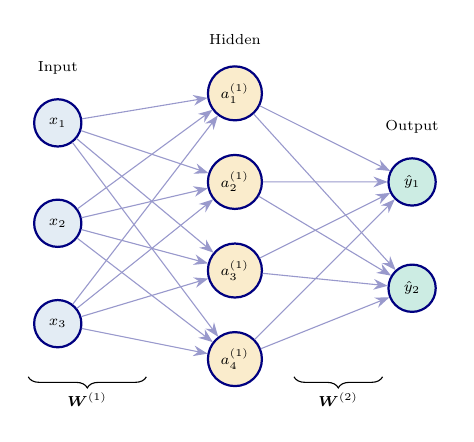
\begin{tikzpicture}[scale=0.75, transform shape,
    neuron/.style={circle, draw=uzhblue, thick, minimum size=8mm},
    arr/.style={-{Stealth[length=1.8mm]}, uzhblue!40}]

    % Input layer
    \node[neuron, fill=softblue!15, font=\scriptsize] (x1) at (0,2.5) {$x_1$};
    \node[neuron, fill=softblue!15, font=\scriptsize] (x2) at (0,0.8) {$x_2$};
    \node[neuron, fill=softblue!15, font=\scriptsize] (x3) at (0,-0.9) {$x_3$};

    % Hidden layer
    \node[neuron, fill=softorange!20, font=\scriptsize] (h1) at (3,3) {$a_1^{(1)}$};
    \node[neuron, fill=softorange!20, font=\scriptsize] (h2) at (3,1.5) {$a_2^{(1)}$};
    \node[neuron, fill=softorange!20, font=\scriptsize] (h3) at (3,0) {$a_3^{(1)}$};
    \node[neuron, fill=softorange!20, font=\scriptsize] (h4) at (3,-1.5) {$a_4^{(1)}$};

    % Output layer
    \node[neuron, fill=softgreen!20, font=\scriptsize] (y1) at (6,1.5) {$\hat{y}_1$};
    \node[neuron, fill=softgreen!20, font=\scriptsize] (y2) at (6,-0.3) {$\hat{y}_2$};

    % Connections
    \foreach \i in {x1,x2,x3} {
        \foreach \j in {h1,h2,h3,h4} { \draw[arr] (\i) -- (\j); }
    }
    \foreach \i in {h1,h2,h3,h4} {
        \foreach \j in {y1,y2} { \draw[arr] (\i) -- (\j); }
    }

    % Labels
    \node[font=\scriptsize, above] at (0,3.2) {Input};
    \node[font=\scriptsize, above] at (3,3.7) {Hidden};
    \node[font=\scriptsize, above] at (6,2.2) {Output};

    % Weight labels
    \draw[decorate, decoration={brace, amplitude=4pt, mirror}] (-0.5,-1.8) -- (1.5,-1.8)
        node[midway, below=4pt, font=\scriptsize]{$\W^{(1)}$};
    \draw[decorate, decoration={brace, amplitude=4pt, mirror}] (4,-1.8) -- (5.5,-1.8)
        node[midway, below=4pt, font=\scriptsize]{$\W^{(2)}$};
\end{tikzpicture}
\end{center}

\column{0.48\textwidth}
\textbf{Hidden layer:}
\begin{align*}
    \z^{(1)} &= \W^{(1)}\x + \bb^{(1)} \\
    \a^{(1)} &= g\!\big(\z^{(1)}\big)
\end{align*}

\textbf{Output layer:}
\begin{align*}
    \z^{(2)} &= \W^{(2)}\a^{(1)} + \bb^{(2)} \\
    \hat{\bm{y}} &= g_{\text{out}}\!\big(\z^{(2)}\big)
\end{align*}

where $\W^{(1)}\in\R^{n_1\times d}$, $\W^{(2)}\in\R^{K\times n_1}$.

\vspace{0.3cm}
{\small The hidden layer creates a \textbf{learned representation} of the input that the output layer then uses for prediction.}
\end{columns}
\end{frame}

% --- Slide 29: Deep Feedforward Network ---
\begin{frame}{Deep Feedforward Networks}
\begin{center}
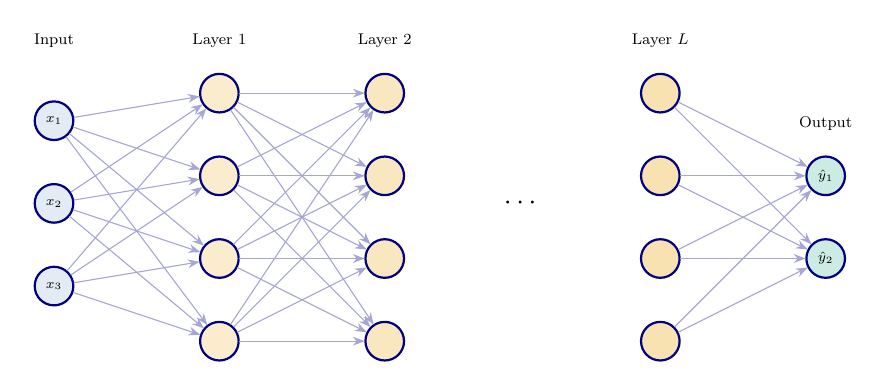
\begin{tikzpicture}[scale=0.7, transform shape,
    neuron/.style={circle, draw=uzhblue, thick, minimum size=7mm},
    arr/.style={-{Stealth[length=1.5mm]}, uzhblue!35}]

    % Input layer
    \foreach \i/\y in {1/2,2/0.5,3/-1} {
        \node[neuron, fill=softblue!15, font=\scriptsize] (x\i) at (0,\y) {$x_\i$};
    }
    % Hidden 1
    \foreach \i/\y in {1/2.5,2/1,3/-0.5,4/-2} {
        \node[neuron, fill=softorange!20, font=\tiny] (h1\i) at (3,\y) {};
    }
    % Hidden 2
    \foreach \i/\y in {1/2.5,2/1,3/-0.5,4/-2} {
        \node[neuron, fill=softorange!25, font=\tiny] (h2\i) at (6,\y) {};
    }
    % Hidden L
    \foreach \i/\y in {1/2.5,2/1,3/-0.5,4/-2} {
        \node[neuron, fill=softorange!30, font=\tiny] (hL\i) at (11,\y) {};
    }
    % Output
    \foreach \i/\y in {1/1,2/-0.5} {
        \node[neuron, fill=softgreen!20, font=\scriptsize] (y\i) at (14,\y) {$\hat{y}_\i$};
    }

    % Dots
    \node[font=\Large] at (8.5,0.5) {$\cdots$};

    % Connections
    \foreach \i in {1,2,3} { \foreach \j in {1,2,3,4} { \draw[arr] (x\i)--(h1\j); }}
    \foreach \i in {1,2,3,4} { \foreach \j in {1,2,3,4} { \draw[arr] (h1\i)--(h2\j); }}
    \foreach \i in {1,2,3,4} { \foreach \j in {1,2} { \draw[arr] (hL\i)--(y\j); }}

    % Layer labels
    \node[font=\footnotesize, above] at (0,3.2) {Input};
    \node[font=\footnotesize, above] at (3,3.2) {Layer 1};
    \node[font=\footnotesize, above] at (6,3.2) {Layer 2};
    \node[font=\footnotesize, above] at (11,3.2) {Layer $L$};
    \node[font=\footnotesize, above] at (14,1.7) {Output};
\end{tikzpicture}
\end{center}

\vspace{0.1cm}
An $L$-layer network computes a nested composition:
\vspace{-0.15cm}
\[
    \boxed{\;\a^{(0)} = \x, \qquad \a^{(\ell)} = g_\ell\!\big(\W^{(\ell)}\a^{(\ell-1)} + \bb^{(\ell)}\big), \qquad f(\x;\bm{\theta}) = \a^{(L)}\;}
\]

{\small Each layer transforms the representation.  For \emph{specific} function classes, \textbf{depth} buys exponentially fewer parameters than width (Telgarsky 2016; Eldan \& Shamir 2016).}
\end{frame}

% --- Slide 30: Universal Approximation ---
\begin{frame}{Universal Approximation Theorem}
\small
\begin{block}{Theorem (Cybenko 1989; Hornik, Stinchcombe \& White 1989)}
Let $g:\R\to\R$ be a bounded, non-constant, continuous activation function.  Then for any continuous function $f:\mathcal{K}\to\R$ on a compact set $\mathcal{K}\subset\R^d$ and any $\varepsilon>0$, there exists a single-hidden-layer network
\[
    F(\x) = \sum_{j=1}^{n_1} v_j\, g\!\big(\w_j^\top\x + b_j\big)
\]
such that $\sup_{\x\in\mathcal{K}} |F(\x) - f(\x)| < \varepsilon$.
\end{block}
\vspace{-0.15cm}

\vspace{0.1cm}
\textbf{Caveats:}
\begin{itemize}\itemsep0pt
    \item The required width $n_1$ may be \textbf{exponentially large} in $d$, and existence $\neq$ efficient learnability.
    \item Practical success suggests \textbf{depth} is a far more efficient parameterization than width alone.
    \item \emphc{Boundedness can be dropped:} density holds iff the activation is \textbf{non-polynomial} (Leshno et al., 1993), and this is what covers \textbf{ReLU}.
\end{itemize}
\end{frame}

% --- Slide 30b: Curse of dimensionality ---
\begin{frame}{Why Networks and Not Grids? The Curse of Dimensionality}
\begin{columns}[T]
\column{0.50\textwidth}
\textbf{A grid dies exponentially.}  Tabulating a function with $N$ points per dimension costs
\[
    N^{d} \quad\text{points.}
\]
{\small With $N=11$: $d=2 \to 121$; $d=5 \to 1.6\times10^5$; $d=10 \to \emphc{2.6\times10^{10}}$.}

\vspace{0.25cm}
\textbf{A network does not.}  Training a net with $P$ parameters on $M$ sampled points costs $O(MP)$, and neither has to grow like $N^d$.

\column{0.47\textwidth}
\begin{block}{Barron (1993)}
\small For functions in the \emph{Barron class}, a one-hidden-layer network with $n_1$ units achieves squared error $O(1/n_1)$, with a constant that does \emphc{not} depend on $d$.
\end{block}

\vspace{0.2cm}
{\footnotesize \emphc{Be honest:} the Barron class is restrictive and $d$ can hide in the constant.  A strong \emph{hint}, not a free lunch, but it is why we sample instead of tabulate.}
\end{columns}

\end{frame}

% --- Slide 31: Geometric View ---
\begin{frame}{A Geometric View: Learning to Untangle}
Neural networks learn \textbf{successive coordinate transformations} that make the data linearly separable.

\vspace{0.3cm}
\begin{center}
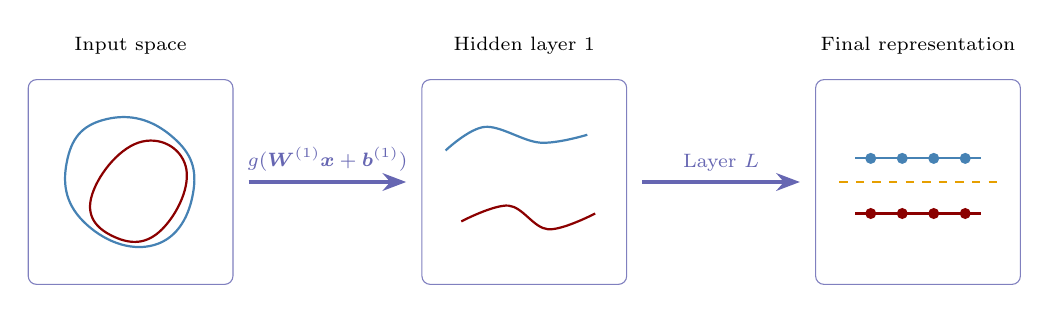
\begin{tikzpicture}[
    box/.style={rectangle, draw=uzhblue!50, rounded corners=3pt,
                minimum width=2.6cm, minimum height=2.6cm, inner sep=0pt},
    arr/.style={-{Stealth[length=3mm]}, very thick, uzhblue!60}
]
    % Panel 1: tangled
    \node[box] (p1) at (0,0) {};
    \node[font=\scriptsize, above] at (0,1.5) {Input space};
    % Draw tangled pattern
    \draw[softblue, thick] plot[smooth cycle, tension=0.8] coordinates {
        (-0.8,0.3) (-0.3,0.8) (0.5,0.6) (0.8,-0.1) (0.3,-0.8) (-0.6,-0.5)};
    \draw[darkred, thick] plot[smooth cycle, tension=0.8] coordinates {
        (-0.5,-0.2) (0.1,0.5) (0.7,0.2) (0.4,-0.6) (-0.2,-0.7)};

    % Arrow 1
    \draw[arr] (1.5,0) -- node[above, font=\scriptsize]{$g(\W^{(1)}\x+\bb^{(1)})$} (3.5,0);

    % Panel 2: partially untangled
    \node[box] (p2) at (5,0) {};
    \node[font=\scriptsize, above] at (5,1.5) {Hidden layer 1};
    \draw[softblue, thick] plot[smooth, tension=0.6] coordinates {
        (4.0,0.4) (4.5,0.7) (5.2,0.5) (5.8,0.6)};
    \draw[darkred, thick] plot[smooth, tension=0.6] coordinates {
        (4.2,-0.5) (4.8,-0.3) (5.3,-0.6) (5.9,-0.4)};

    % Arrow 2
    \draw[arr] (6.5,0) -- node[above, font=\scriptsize]{Layer $L$} (8.5,0);

    % Panel 3: linearly separable
    \node[box] (p3) at (10,0) {};
    \node[font=\scriptsize, above] at (10,1.5) {Final representation};
    % Separated
    \draw[softblue, thick] (9.2,0.3) -- (10.8,0.3);
    \fill[softblue] (9.4,0.3) circle (2pt);
    \fill[softblue] (9.8,0.3) circle (2pt);
    \fill[softblue] (10.2,0.3) circle (2pt);
    \fill[softblue] (10.6,0.3) circle (2pt);
    \draw[darkred, thick] (9.2,-0.4) -- (10.8,-0.4);
    \fill[darkred] (9.4,-0.4) circle (2pt);
    \fill[darkred] (9.8,-0.4) circle (2pt);
    \fill[darkred] (10.2,-0.4) circle (2pt);
    \fill[darkred] (10.6,-0.4) circle (2pt);
    % Separating line
    \draw[softorange, thick, dashed] (9.0,0) -- (11.0,0);
\end{tikzpicture}
\end{center}

\vspace{0.2cm}
{\small Analogy (Chollet, 2017): imagine crumpling two sheets of colored paper into a ball. A neural network learns how to smooth them out again, layer by layer, until a simple linear classifier can separate the colors.}
\end{frame}

% ============================================================================
% PART 4: TRAINING NEURAL NETWORKS
% ============================================================================

\section{Training Neural Networks}

% --- Section Divider ---
\begin{frame}{}
\begin{center}
{\Huge \textcolor{uzhblue}{Part III}}\\[0.8em]
{\LARGE Training: Loss, Gradients, and Optimization}
\end{center}
\end{frame}

% --- Slide 33: Loss Functions ---
\begin{frame}{Loss Functions}
The loss function $J(\bm{\theta})$ measures how far predictions $\hat{\bm{y}}$ are from targets $\bm{y}$.

\vspace{0.4cm}
\begin{columns}[T]
\column{0.48\textwidth}
\begin{block}{Regression: Mean Squared Error}
\[
    J(\bm{\theta}) = \frac{1}{2n}\sum_{i=1}^{n}\big(y^{(i)} - f(\x^{(i)};\bm{\theta})\big)^{2}
\]
Penalizes large deviations quadratically.
\end{block}

\column{0.48\textwidth}
\begin{block}{Classification: Cross-Entropy}
{\footnotesize
\[
    J = -\frac{1}{n}\sum_{i=1}^{n}\!\Big[y^{(i)}\!\log\hat{y}^{(i)} + (1{-}y^{(i)})\log(1{-}\hat{y}^{(i)})\Big]
\]}%
\vspace{-0.3cm}

For binary labels $y\in\{0,1\}$.
\end{block}
\end{columns}

\vspace{0.3cm}
\textbf{Multiclass} ($K$ classes): use softmax output $\hat{y}_k = e^{z_k}\big/\sum_j e^{z_j}$ and categorical cross-entropy:
$J = -\frac{1}{n}\sum_{i}\sum_{k} y_k^{(i)}\log \hat{y}_k^{(i)}$.
\end{frame}

% --- Slide 34: Choosing a Loss Function ---
\begin{frame}{Choosing a Loss Function}
{\small Beyond MSE, with residual $r = y - \hat{y}$: \textbf{Huber} is quadratic near zero and linear in the tails, and the \textbf{quantile} (pinball) loss $\rho_\tau(r) = r\,(\tau - \mathbf{1}[r<0])$ is deliberately asymmetric.}

\vspace{0.15cm}
\begin{center}
{\footnotesize
\renewcommand{\arraystretch}{1.2}
\begin{tabular}{lccl}
\toprule
\textbf{Loss} & \textbf{Sensitivity to outliers} & \textbf{Symmetry} & \textbf{Use case} \\
\midrule
MSE      & High & Symmetric           & Default regression \\
Huber    & Low  & Symmetric           & Robust regression \\
Quantile & Low  & \textbf{Asymmetric} & Risk, VaR, tails \\
\bottomrule
\end{tabular}
}%
\end{center}

\vspace{0.2cm}
\begin{exampleblock}{Why this matters in economics and finance}
\small
Tail risks are often more important than average performance.
\textbf{Quantile loss} lets the model focus on getting worst-case predictions right,
directly producing \textbf{Value-at-Risk} estimates.
{\footnotesize (Expected Shortfall is \emph{not} elicitable on its own; it needs the joint VaR/ES scoring function of Fissler \& Ziegel, 2016.)}
\end{exampleblock}

\vspace{0.1cm}
{\footnotesize \textbf{References:} Huber (1964), Koenker \& Bassett (1978).}
\end{frame}

% --- Slide 35: Gradient Descent Idea ---
\begin{frame}{Gradient Descent: The Idea}
\begin{columns}[T]
\column{0.48\textwidth}
\textbf{Goal:} $\bm{\theta}^{*} = \argmin_{\bm{\theta}} J(\bm{\theta})$.  Step downhill from a random start, with learning rate $\eta>0$:
\vspace{-0.15cm}
\[
    \bm{\theta} \;\leftarrow\; \bm{\theta} - \eta\,\nabla_{\!\bm{\theta}} J(\bm{\theta}).
\]
\vspace{-0.45cm}

\begin{block}{Algorithm}
\small Initialize $\bm{\theta}\sim\mathcal{N}(\bm{0},\sigma^2\bm{I})$, then repeat:
\vspace{-0.15cm}
\[
    \bm{g} \leftarrow \nabla_{\!\bm{\theta}} J(\bm{\theta}), \qquad \bm{\theta} \leftarrow \bm{\theta} - \eta\,\bm{g}.
\]
\vspace{-0.5cm}
\end{block}

{\footnotesize Each step costs $O(N)$ over the whole training set, and the iteration converges to a \textbf{stationary point}, usually a \emph{saddle} (Dauphin et al.\ 2014).}

\column{0.48\textwidth}
\begin{center}
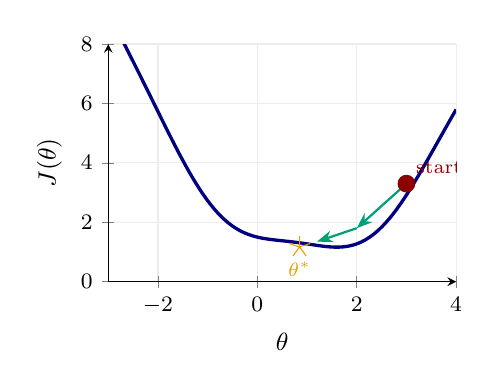
\begin{tikzpicture}
\begin{axis}[
    width=6.0cm, height=4.6cm,
    xlabel={$\theta$}, ylabel={$J(\theta)$},
    xmin=-3, xmax=4, ymin=0, ymax=8,
    grid=major, grid style={gray!15},
    axis lines=left,
    ytick={0,2,4,6,8},
]
    % Loss curve
    \addplot[very thick, uzhblue, domain=-3:4, samples=100]{0.5*(x-1)^2 + 0.3*sin(deg(x*2)) + 1};
    % Starting point
    \addplot[only marks, mark=*, mark size=3pt, darkred] coordinates {(3, 3.3)};
    \node[font=\scriptsize, darkred, above right] at (axis cs:3,3.3) {start};
    % Arrow showing descent
    \draw[-{Stealth[length=2mm]}, thick, softgreen] (axis cs:3,3.3) -- (axis cs:2,1.8);
    \draw[-{Stealth[length=2mm]}, thick, softgreen] (axis cs:2,1.8) -- (axis cs:1.2,1.35);
    % Minimum
    \addplot[only marks, mark=star, mark size=4pt, softorange] coordinates {(0.85, 1.17)};
    \node[font=\scriptsize, softorange, below] at (axis cs:0.85,1.0) {$\theta^*$};
\end{axis}
\end{tikzpicture}
\end{center}
\end{columns}
\end{frame}

% --- Slide 37: SGD ---
\begin{frame}{Stochastic Gradient Descent (SGD)}
\textbf{Idea:} approximate the full gradient with a cheap estimate from a small subset of data.

\vspace{0.1cm}
\begin{columns}[T]
\column{0.48\textwidth}
\begin{block}{Single-sample SGD}
\small Pick one random example $(\x^{(i)},y^{(i)})$:
\[
    \bm{\theta} \leftarrow \bm{\theta} - \eta\,\nabla_{\!\bm{\theta}} J_i(\bm{\theta})
\]
Cheap but noisy.
\end{block}

\column{0.48\textwidth}
\begin{block}{Mini-batch SGD}
\small Sample a batch $\mathcal{B}$ of $B$ examples:
\[
    \bm{\theta} \leftarrow \bm{\theta} - \frac{\eta}{B}\sum_{k\in\mathcal{B}} \nabla_{\!\bm{\theta}} J_k(\bm{\theta})
\]
Reduces variance; enables GPU parallelism.
\end{block}
\end{columns}

\vspace{0.15cm}
{\footnotesize\textbf{Why does this work?} The mini-batch gradient is an \textbf{unbiased estimate} of the full gradient, $\E{\tfrac{1}{B}\sum_{k\in\mathcal{B}}\nabla J_k} = \nabla J$.}

{\small Unbiasedness \emph{plus} a decaying step size, $\sum_t\eta_t=\infty$ and $\sum_t\eta_t^2<\infty$, gives convergence (Robbins \& Monro, 1951).  With a \emphc{constant} $\eta$, SGD instead hovers in an $O(\eta)$ neighbourhood of the optimum, hence learning-rate decay.}
\end{frame}

% --- Slide 38: Mini-batches and Epochs ---
\begin{frame}{Mini-Batches and Epochs}
\begin{center}
\resizebox{0.97\textwidth}{!}{%
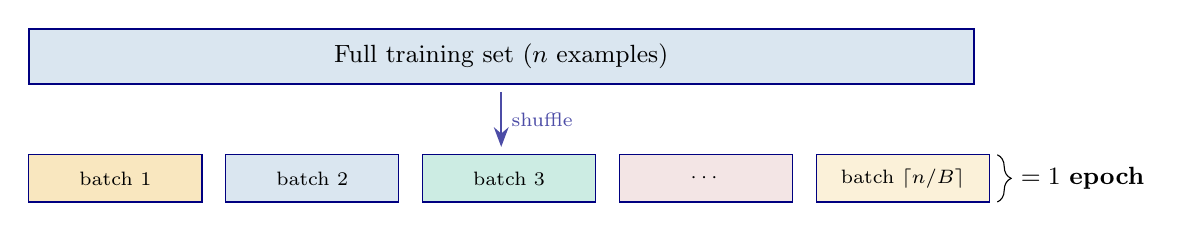
\begin{tikzpicture}[
    box/.style={rectangle, draw=uzhblue, rounded corners=3pt, minimum height=8mm, font=\small, inner sep=4pt},
    arr/.style={-{Stealth[length=2.5mm]}, thick, uzhblue!70}
]
    % Training data bar
    \fill[softblue!20] (0,0) rectangle (12,0.7);
    \draw[uzhblue, thick] (0,0) rectangle (12,0.7);
    \node[font=\small] at (6, 0.35) {Full training set ($n$ examples)};

    % Shuffle arrow
    \draw[arr] (6,-0.1) -- (6,-0.8) node[right, font=\scriptsize, pos=0.5]{shuffle};

    % Mini-batches
    \foreach \i/\c in {0/softorange!25, 2.5/softblue!20, 5/softgreen!20, 7.5/darkred!10, 10/softorange!15} {
        \fill[\c] (\i,-1.5) rectangle (\i+2.2,-0.9);
        \draw[uzhblue] (\i,-1.5) rectangle (\i+2.2,-0.9);
    }
    \node[font=\scriptsize] at (1.1,-1.2) {batch 1};
    \node[font=\scriptsize] at (3.6,-1.2) {batch 2};
    \node[font=\scriptsize] at (6.1,-1.2) {batch 3};
    \node[font=\scriptsize] at (8.6,-1.2) {$\cdots$};
    \node[font=\scriptsize] at (11.1,-1.2) {batch $\lceil n/B\rceil$};

    % Brace for epoch
    \draw[decorate, decoration={brace, amplitude=5pt}] (12.3,-0.9) -- (12.3,-1.5)
        node[midway, right=5pt, font=\small]{$= 1$ \textbf{epoch}};
\end{tikzpicture}}
\end{center}

\vspace{0.5cm}
\begin{itemize}
    \item One \textbf{epoch} = one complete pass through the training set.
    \begin{itemize}\item[\textendash] {\footnotesize When data are \emph{simulated} rather than fixed, as in the next lecture, there is no epoch: you draw fresh mini-batches forever.}\end{itemize}
    \item Typical batch sizes: $B \in \{32, 64, 128, 256\}$.
    \item Benefits of mini-batches:
    \begin{itemize}
        \item[\textendash] Smoother convergence than single-sample SGD.
        \item[\textendash] Efficient use of GPU parallelism.
        \item[\textendash] Implicit regularization from gradient noise.
    \end{itemize}
\end{itemize}
\end{frame}

% --- Slide 39: Backpropagation Key Idea ---
\begin{frame}{Backpropagation: The Key Idea}
\textbf{Problem:} how do we compute $\frac{\partial J}{\partial \W^{(\ell)}}$ for each layer $\ell$?

\vspace{0.3cm}
\textbf{Answer:} the \textbf{chain rule} of calculus, applied systematically.

\vspace{0.4cm}
\begin{center}
\resizebox{\textwidth}{!}{%
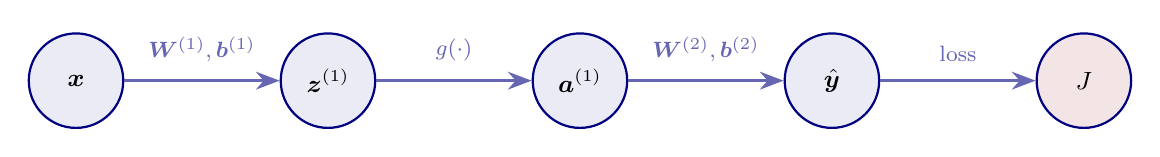
\begin{tikzpicture}[
    node/.style={circle, draw=uzhblue, thick, minimum size=12mm, fill=uzhblue!8, font=\small},
    arr/.style={-{Stealth[length=3mm]}, very thick, uzhblue!60}
]
    \node[node] (x) at (0,0) {$\x$};
    \node[node] (z1) at (3.2,0) {$\z^{(1)}$};
    \node[node] (a1) at (6.4,0) {$\a^{(1)}$};
    \node[node] (yhat) at (9.6,0) {$\hat{\bm{y}}$};
    \node[node, fill=darkred!10] (J) at (12.8,0) {$J$};

    \draw[arr] (x) -- node[above=3pt, font=\footnotesize]{$\W^{(1)},\bb^{(1)}$} (z1);
    \draw[arr] (z1) -- node[above=3pt, font=\footnotesize]{$g(\cdot)$} (a1);
    \draw[arr] (a1) -- node[above=3pt, font=\footnotesize]{$\W^{(2)},\bb^{(2)}$} (yhat);
    \draw[arr] (yhat) -- node[above=3pt, font=\footnotesize]{loss} (J);
\end{tikzpicture}}
\end{center}

\vspace{0.3cm}
\[
    \frac{\partial J}{\partial \W^{(1)}} = \underbrace{\frac{\partial J}{\partial \hat{\bm{y}}}}_{\footnotesize\text{output error}} \cdot \underbrace{\frac{\partial \hat{\bm{y}}}{\partial \a^{(1)}}}_{\footnotesize\W^{(2)}} \cdot \underbrace{\frac{\partial \a^{(1)}}{\partial \z^{(1)}}}_{\footnotesize g'(\z^{(1)})} \cdot \underbrace{\frac{\partial \z^{(1)}}{\partial \W^{(1)}}}_{\footnotesize\x}
\]
\end{frame}

% --- Slide 41: Backpropagation Backward Pass ---
\begin{frame}{Backpropagation: The Backward Pass}
{\footnotesize \emphc{Forward pass first:} evaluate $\z^{(\ell)}, \a^{(\ell)}$ layer by layer and \textbf{store them}, because the backward pass needs them.}

\vspace{0.1cm}
Define the \textbf{error signal} at layer $\ell$: $\;\bm{\delta}^{(\ell)} \equiv \partial J/\partial \z^{(\ell)} \in \R^{n_\ell}$.

\textbf{Output layer} ($\ell = L$):
\[
    \bm{\delta}^{(L)} = \nabla_{\!\z^{(L)}} J = \frac{\partial J}{\partial \hat{\bm{y}}}\odot g_{\text{out}}'(\z^{(L)})
\]

\textbf{Hidden layers} ($\ell = L{-}1, \dots, 1$), propagating the error \textit{backward}:
\[
    \boxed{\bm{\delta}^{(\ell)} = \big(\W^{(\ell+1)}\big)^{\!\top}\bm{\delta}^{(\ell+1)} \;\odot\; g'\!\big(\z^{(\ell)}\big)}
\]

\textbf{Parameter gradients:}
\vspace{-0.15cm}
\[
    \frac{\partial J}{\partial \W^{(\ell)}} = \bm{\delta}^{(\ell)}\big(\a^{(\ell-1)}\big)^{\!\top}, \qquad
    \frac{\partial J}{\partial \bb^{(\ell)}} = \bm{\delta}^{(\ell)}
\]
\vspace{-0.5cm}


{\footnotesize $\odot$ is the element-wise product.  The form of $\bm{\delta}^{(L)}$ above assumes a \emph{coordinatewise} $g_{\text{out}}$; for \textbf{softmax $+$ cross-entropy} (and linear $+$ MSE) it collapses to $\bm{\delta}^{(L)} = \hat{\bm{y}} - \bm{y}$.}
\end{frame}

% --- Slide 41b: Autodiff bridge ---
\begin{frame}{Backpropagation Is Automatic Differentiation}
\textbf{You will never implement the previous slide by hand.}  Backpropagation is exactly \emphc{reverse-mode automatic differentiation}, and every framework does it for you.

\vspace{0.25cm}
\begin{itemize}\itemsep3pt
    \item TensorFlow / PyTorch / JAX record the \textbf{computation graph} as you evaluate the forward pass, then walk it backwards.
    \item They return $\nabla_{\bm{\theta}}$ of \emphc{any scalar} you can build from $\bm{\theta}$, and the code does not care where that scalar came from.
    \item Cost: one backward pass $\approx$ 2--3$\times$ one forward pass, \textbf{independent of the number of parameters}.
\end{itemize}

\vspace{0.25cm}
\begin{exampleblock}{The hinge of this whole summer school}
\small Nothing in autodiff requires the loss to come from \emph{labels}; it only has to be a differentiable function of $\bm{\theta}$.  So we can put an \emphc{Euler-equation residual} in the loss and get $\nabla_{\bm{\theta}}$ for free.  That is exactly what \textbf{Deep Equilibrium Nets} do next.
\end{exampleblock}
\end{frame}

% --- Slide 42: Learning Rate ---
\begin{frame}{The Learning Rate}
\begin{center}
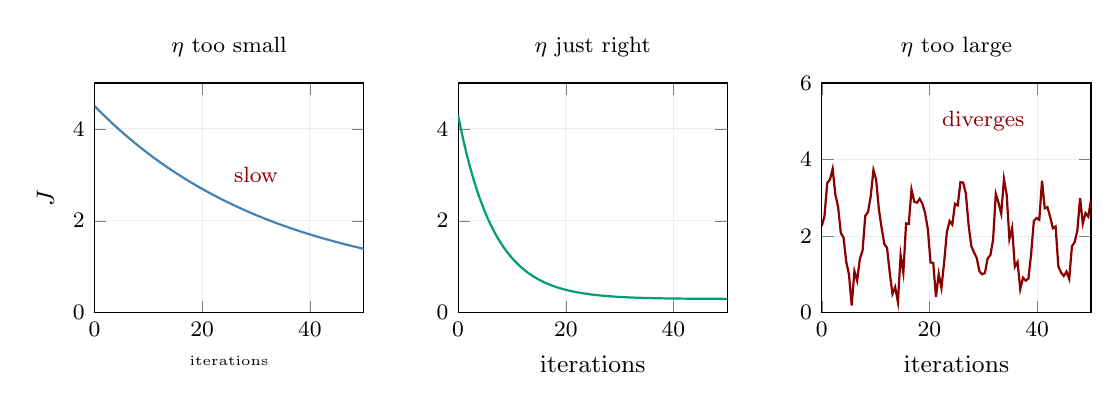
\begin{tikzpicture}
\begin{axis}[
    name=plotL,
    width=5cm, height=4.5cm,
    title={\footnotesize $\eta$ too small},
    xlabel={iterations}, ylabel={$J$},
    xlabel style={font=\tiny},    xmin=0, xmax=50, ymin=0, ymax=5,
    grid=major, grid style={gray!15},
]
    \addplot[thick, softblue, domain=0:50, samples=100]{4*exp(-0.03*x)+0.5};
    \node[font=\footnotesize, darkred] at (axis cs:30,3) {slow};
\end{axis}

\begin{axis}[
    at={($(plotL.east)+(1.2cm,0)$)}, anchor=west,
    name=plotM,
    width=5cm, height=4.5cm,
    title={\footnotesize $\eta$ just right},
    xlabel={iterations},
    xmin=0, xmax=50, ymin=0, ymax=5,
    grid=major, grid style={gray!15},
]
    \addplot[thick, softgreen, domain=0:50, samples=100]{4*exp(-0.15*x)+0.3};
\end{axis}

\begin{axis}[
    at={($(plotM.east)+(1.2cm,0)$)}, anchor=west,
    width=5cm, height=4.5cm,
    title={\footnotesize $\eta$ too large},
    xlabel={iterations},
    xmin=0, xmax=50, ymin=0, ymax=6,
    grid=major, grid style={gray!15},
]
    \addplot[thick, darkred, domain=0:50, samples=100]{2+1.5*sin(deg(x*0.8))*exp(-0.01*x)+0.5*rand};
    \node[font=\footnotesize, darkred] at (axis cs:30,5) {diverges};
\end{axis}
\end{tikzpicture}
\end{center}

\vspace{0.3cm}
\begin{itemize}
    \item \textbf{Too small:} slow convergence, may get stuck in poor local minima.
    \item \textbf{Too large:} oscillation or divergence, overshooting the minimum.
    \item \textbf{Solution:} use \textbf{adaptive learning rates} that adjust automatically.
\end{itemize}
\end{frame}

% --- Slide 43: Adaptive Optimizers ---
\begin{frame}{Adaptive Optimizers}
{\footnotesize Plain SGD uses one learning rate for every parameter.  \textbf{Momentum} averages the gradient over time to damp oscillations.  \textbf{Adam} goes further and gives each coordinate its own step.}

\vspace{0.2cm}
\begin{block}{Adam (Kingma \& Ba, 2015)}
\small
Track a first and a second moment, correct their bias, then rescale:
\begin{align*}
    \bm{m}_t &= \beta_1\bm{m}_{t-1} + (1-\beta_1)\nabla J, &
    \bm{v}_t &= \beta_2\bm{v}_{t-1} + (1-\beta_2)(\nabla J)^2, \\[2pt]
    \hat{\bm{m}}_t &= \bm{m}_t/(1-\beta_1^t), \quad
    \hat{\bm{v}}_t = \bm{v}_t/(1-\beta_2^t), &
    \bm{\theta}_{t+1} &= \bm{\theta}_t - \eta\,\frac{\hat{\bm{m}}_t}{\sqrt{\hat{\bm{v}}_t} + \varepsilon}
\end{align*}
\end{block}

\vspace{0.15cm}
\begin{exampleblock}{What to actually do}
\centering\small Use \textbf{Adam} with the defaults $\beta_1 = 0.9$, $\beta_2 = 0.999$, $\varepsilon = 10^{-8}$; tune only $\eta$, starting at $10^{-3}$.
\end{exampleblock}

\vspace{0.05cm}
{\footnotesize RMSProp is the same idea using only the second moment; for true weight decay, use \textbf{AdamW}.}
\end{frame}

% --- Slide 44: Initialization and Gradient Pathologies (merged) ---
\begin{frame}{Weight Initialization}
\textbf{Why not initialize all weights to zero?} Every neuron would compute the same output, receive the same gradient, and the symmetry would never break.

\vspace{0.4cm}
\begin{columns}[T]
\column{0.48\textwidth}
\begin{block}{Xavier / Glorot (2010): sigmoid, tanh}
\[
    W_{ij}^{(\ell)} \sim \mathcal{N}\!\left(0,\; \tfrac{2}{n_{\ell-1} + n_{\ell}}\right)
\]
\end{block}

\column{0.48\textwidth}
\begin{block}{He (2015): ReLU}
\[
    W_{ij}^{(\ell)} \sim \mathcal{N}\!\left(0,\; \tfrac{2}{n_{\ell-1}}\right)
\]
\end{block}
\end{columns}

\vspace{0.25cm}
{\small Both keep activation variance roughly constant across layers; biases start at zero.}

\vspace{0.25cm}
\begin{alertblock}{Standardize your inputs}
\small These variances are \emph{derived} assuming zero-mean, unit-variance inputs.  An economic state vector mixing capital, TFP and portfolio shares silently breaks that.
\end{alertblock}
\end{frame}

% --- Vanishing / exploding gradients ---
\begin{frame}{Vanishing and Exploding Gradients}
\begin{columns}[T]
\column{0.52\textwidth}
{\small The backward pass multiplies a factor through every layer,
\vspace{-0.1cm}
\[
    \bm{\delta}^{(\ell)} = \big(\W^{(\ell+1)}\big)^{\!\top}\bm{\delta}^{(\ell+1)}\odot g'(\z^{(\ell)}),
\]
\vspace{-0.5cm}

so the per-layer growth factor is $\|\W^{(\ell+1)}\|\cdot|g'(\z^{(\ell)})|$.}

\vspace{0.1cm}
\begin{itemize}\itemsep2pt
    \item {\small Sigmoid has $g'\le\tfrac14$, so with $\|\W\|\approx1$ the product decays like $4^{-L}$, the \textbf{vanishing gradient} case.}
    \item {\small Large $\|\W\|$ gives the opposite: \textbf{exploding gradients}.}
\end{itemize}

\vspace{0.05cm}
{\footnotesize\textbf{Remedies:} ReLU, scaled initialization, \textbf{residual connections} (He et al.\ 2016), batch norm, gradient clipping.}

\column{0.45\textwidth}
\begin{center}
{\small\textbf{Sigmoid saturation zones}}
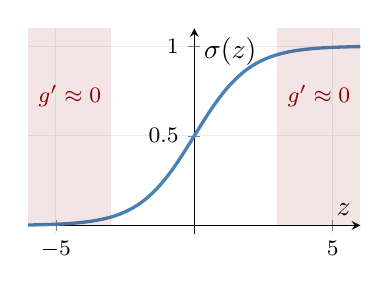
\begin{tikzpicture}
\begin{axis}[
    width=5.8cm, height=4.2cm,
    xlabel={$z$}, ylabel={$\sigma(z)$},
    xmin=-6, xmax=6, ymin=-0.05, ymax=1.1,
    grid=major, grid style={gray!15},
    axis lines=middle,
]
    \addplot[very thick, softblue, domain=-6:6, samples=100]{1/(1+exp(-x))};
    \fill[darkred, opacity=0.1] (axis cs:-6,0) rectangle (axis cs:-3,1.1);
    \fill[darkred, opacity=0.1] (axis cs:3,0) rectangle (axis cs:6,1.1);
    \node[font=\footnotesize, darkred] at (axis cs:-4.5,0.72) {$g' \approx 0$};
    \node[font=\footnotesize, darkred] at (axis cs:4.5,0.72) {$g' \approx 0$};
\end{axis}
\end{tikzpicture}
\end{center}
\end{columns}
\end{frame}

% --- Slide 45: Loss Landscape ---
\begin{frame}{Loss Landscapes of Neural Networks}
\begin{columns}[T]
\column{0.52\textwidth}
\begin{center}
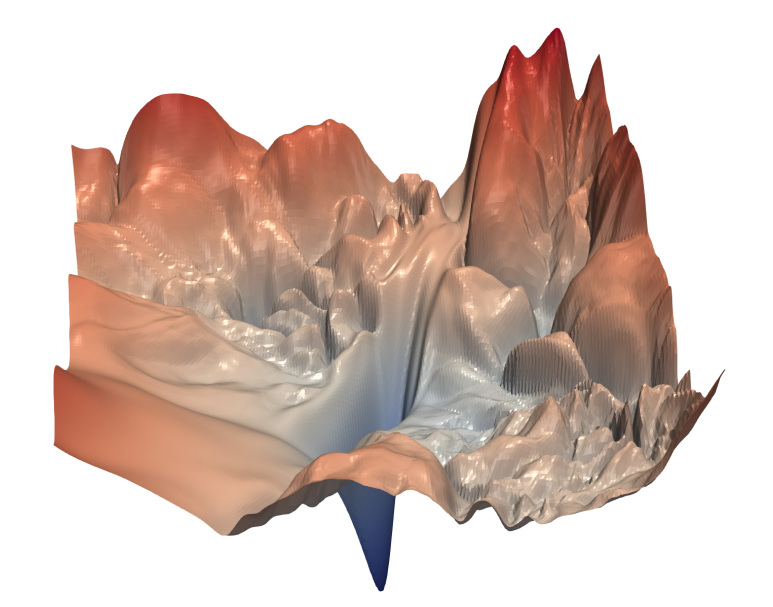
\includegraphics[width=0.94\textwidth]{figures/landscape.png}
\end{center}

\column{0.45\textwidth}
The loss surface of a deep network is highly non-convex:
\begin{itemize}\itemsep1pt
    \item Many \textbf{local minima} and \textbf{saddle points}
    \item SGD noise helps escape poor ones
\end{itemize}

\vspace{0.2cm}
{\footnotesize Li et al.\ (2018) \emph{visualize} these surfaces.  A widely-held \emph{hypothesis} says flat minima generalize better (Hochreiter \& Schmidhuber 1997; Keskar et al.\ 2017), but sharpness is reparameterization-dependent (Dinh et al.\ 2017), so treat it as intuition rather than theorem.}
\end{columns}
\end{frame}

% ============================================================================
% PART 5: GENERALIZATION AND REGULARIZATION
% ============================================================================

\section{Generalization and Regularization}

% --- Section Divider ---
\begin{frame}{}
\begin{center}
{\Huge \textcolor{uzhblue}{Part IV}}\\[0.8em]
{\LARGE Generalization and Regularization}
\end{center}
\end{frame}

% --- Slide 46: Overfitting ---
\begin{frame}{Overfitting and Underfitting}
\begin{center}
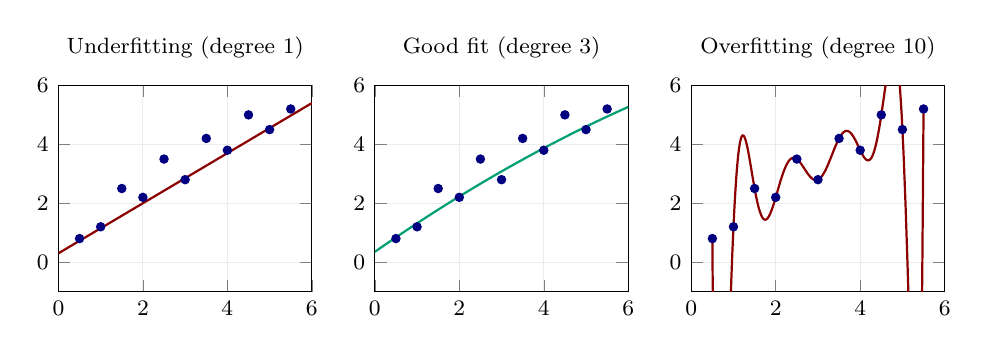
\begin{tikzpicture}
% Panel 1: Underfitting
\begin{axis}[
    name=p1,
    width=4.8cm, height=4.2cm,
    title={\footnotesize Underfitting (degree 1)},
    xmin=0, xmax=6, ymin=-1, ymax=6,
    grid=major, grid style={gray!15},
]
    \addplot[only marks, mark=*, mark size=1.5pt, uzhblue] coordinates {
        (0.5,0.8) (1,1.2) (1.5,2.5) (2,2.2) (2.5,3.5) (3,2.8) (3.5,4.2) (4,3.8) (4.5,5) (5,4.5) (5.5,5.2)
    };
    \addplot[thick, darkred, domain=0:6, samples=2]{0.3+0.85*x};
\end{axis}

% Panel 2: Good fit
\begin{axis}[
    at={($(p1.east)+(0.8cm,0)$)}, anchor=west,
    name=p2,
    width=4.8cm, height=4.2cm,
    title={\footnotesize Good fit (degree 3)},
    xmin=0, xmax=6, ymin=-1, ymax=6,
    grid=major, grid style={gray!15},
]
    \addplot[only marks, mark=*, mark size=1.5pt, uzhblue] coordinates {
        (0.5,0.8) (1,1.2) (1.5,2.5) (2,2.2) (2.5,3.5) (3,2.8) (3.5,4.2) (4,3.8) (4.5,5) (5,4.5) (5.5,5.2)
    };
    \addplot[thick, softgreen, domain=0:6, samples=100]{0.35+1.0*x-0.03*x^2};
\end{axis}

% Panel 3: Overfitting
\begin{axis}[
    at={($(p2.east)+(0.8cm,0)$)}, anchor=west,
    width=4.8cm, height=4.2cm,
    title={\footnotesize Overfitting (degree 10)},
    xmin=0, xmax=6, ymin=-1, ymax=6,
    grid=major, grid style={gray!15},
]
    \addplot[only marks, mark=*, mark size=1.5pt, uzhblue] coordinates {
        (0.5,0.8) (1,1.2) (1.5,2.5) (2,2.2) (2.5,3.5) (3,2.8) (3.5,4.2) (4,3.8) (4.5,5) (5,4.5) (5.5,5.2)
    };
    % true degree-10 interpolant through all 11 points: hits every one,
    % and oscillates violently between them (Runge phenomenon)
    \addplot[thick, darkred] coordinates {(0.500,0.800) (0.516,-2.274) (0.531,-4.000) (0.547,-4.000) (0.563,-4.000) (0.578,-4.000) (0.594,-4.000) (0.610,-4.000) (0.625,-4.000) (0.641,-4.000) (0.657,-4.000) (0.672,-4.000) (0.688,-4.000) (0.704,-4.000) (0.719,-4.000) (0.735,-4.000) (0.751,-4.000) (0.766,-4.000) (0.782,-4.000) (0.798,-4.000) (0.813,-4.000) (0.829,-4.000) (0.845,-4.000) (0.861,-4.000) (0.876,-3.767) (0.892,-3.027) (0.908,-2.314) (0.923,-1.631) (0.939,-0.980) (0.955,-0.366) (0.970,0.211) (0.986,0.750) (1.002,1.248) (1.017,1.706) (1.033,2.124) (1.049,2.501) (1.064,2.839) (1.080,3.138) (1.096,3.399) (1.111,3.623) (1.127,3.812) (1.143,3.968) (1.158,4.092) (1.174,4.185) (1.190,4.251) (1.205,4.290) (1.221,4.304) (1.237,4.296) (1.252,4.268) (1.268,4.220) (1.284,4.157) (1.299,4.078) (1.315,3.987) (1.331,3.885) (1.346,3.773) (1.362,3.653) (1.378,3.528) (1.393,3.398) (1.409,3.265) (1.425,3.131) (1.440,2.996) (1.456,2.862) (1.472,2.730) (1.487,2.601) (1.503,2.475) (1.519,2.355) (1.534,2.240) (1.550,2.131) (1.566,2.029) (1.582,1.934) (1.597,1.847) (1.613,1.768) (1.629,1.697) (1.644,1.635) (1.660,1.581) (1.676,1.537) (1.691,1.500) (1.707,1.473) (1.723,1.454) (1.738,1.444) (1.754,1.441) (1.770,1.447) (1.785,1.460) (1.801,1.481) (1.817,1.508) (1.832,1.542) (1.848,1.582) (1.864,1.628) (1.879,1.680) (1.895,1.736) (1.911,1.796) (1.926,1.861) (1.942,1.928) (1.958,1.999) (1.973,2.072) (1.989,2.147) (2.005,2.223) (2.020,2.300) (2.036,2.378) (2.052,2.456) (2.067,2.533) (2.083,2.610) (2.099,2.686) (2.114,2.760) (2.130,2.832) (2.146,2.902) (2.161,2.969) (2.177,3.033) (2.193,3.094) (2.208,3.152) (2.224,3.207) (2.240,3.257) (2.255,3.304) (2.271,3.347) (2.287,3.386) (2.303,3.420) (2.318,3.450) (2.334,3.476) (2.350,3.497) (2.365,3.515) (2.381,3.528) (2.397,3.537) (2.412,3.542) (2.428,3.542) (2.444,3.540) (2.459,3.533) (2.475,3.523) (2.491,3.510) (2.506,3.493) (2.522,3.474) (2.538,3.452) (2.553,3.427) (2.569,3.400) (2.585,3.372) (2.600,3.342) (2.616,3.310) (2.632,3.277) (2.647,3.244) (2.663,3.209) (2.679,3.175) (2.694,3.140) (2.710,3.106) (2.726,3.072) (2.741,3.039) (2.757,3.008) (2.773,2.977) (2.788,2.948) (2.804,2.921) (2.820,2.895) (2.835,2.872) (2.851,2.851) (2.867,2.833) (2.882,2.818) (2.898,2.805) (2.914,2.795) (2.929,2.789) (2.945,2.785) (2.961,2.785) (2.976,2.789) (2.992,2.795) (3.008,2.805) (3.024,2.819) (3.039,2.836) (3.055,2.856) (3.071,2.880) (3.086,2.907) (3.102,2.937) (3.118,2.970) (3.133,3.006) (3.149,3.045) (3.165,3.086) (3.180,3.130) (3.196,3.177) (3.212,3.225) (3.227,3.275) (3.243,3.327) (3.259,3.381) (3.274,3.436) (3.290,3.491) (3.306,3.548) (3.321,3.605) (3.337,3.662) (3.353,3.719) (3.368,3.775) (3.384,3.831) (3.400,3.886) (3.415,3.940) (3.431,3.993) (3.447,4.043) (3.462,4.092) (3.478,4.139) (3.494,4.183) (3.509,4.225) (3.525,4.263) (3.541,4.299) (3.556,4.331) (3.572,4.360) (3.588,4.386) (3.603,4.407) (3.619,4.425) (3.635,4.439) (3.650,4.449) (3.666,4.455) (3.682,4.457) (3.697,4.454) (3.713,4.448) (3.729,4.438) (3.745,4.423) (3.760,4.405) (3.776,4.383) (3.792,4.358) (3.807,4.329) (3.823,4.297) (3.839,4.262) (3.854,4.224) (3.870,4.184) (3.886,4.141) (3.901,4.097) (3.917,4.051) (3.933,4.005) (3.948,3.957) (3.964,3.909) (3.980,3.861) (3.995,3.814) (4.011,3.768) (4.027,3.723) (4.042,3.680) (4.058,3.639) (4.074,3.601) (4.089,3.567) (4.105,3.536) (4.121,3.510) (4.136,3.488) (4.152,3.472) (4.168,3.461) (4.183,3.456) (4.199,3.457) (4.215,3.466) (4.230,3.481) (4.246,3.504) (4.262,3.535) (4.277,3.574) (4.293,3.621) (4.309,3.676) (4.324,3.740) (4.340,3.813) (4.356,3.894) (4.371,3.983) (4.387,4.080) (4.403,4.186) (4.418,4.300) (4.434,4.421) (4.450,4.549) (4.466,4.684) (4.481,4.824) (4.497,4.970) (4.513,5.121) (4.528,5.275) (4.544,5.432) (4.560,5.591) (4.575,5.751) (4.591,5.910) (4.607,6.067) (4.622,6.221) (4.638,6.370) (4.654,6.514) (4.669,6.650) (4.685,6.776) (4.701,6.891) (4.716,6.994) (4.732,7.082) (4.748,7.153) (4.763,7.206) (4.779,7.238) (4.795,7.248) (4.810,7.233) (4.826,7.193) (4.842,7.124) (4.857,7.025) (4.873,6.895) (4.889,6.731) (4.904,6.533) (4.920,6.298) (4.936,6.026) (4.951,5.715) (4.967,5.365) (4.983,4.975) (4.998,4.545) (5.014,4.075) (5.030,3.566) (5.045,3.019) (5.061,2.435) (5.077,1.815) (5.092,1.163) (5.108,0.481) (5.124,-0.226) (5.139,-0.953) (5.155,-1.697) (5.171,-2.449) (5.187,-3.204) (5.202,-3.952) (5.218,-4.000) (5.234,-4.000) (5.249,-4.000) (5.265,-4.000) (5.281,-4.000) (5.296,-4.000) (5.312,-4.000) (5.328,-4.000) (5.343,-4.000) (5.359,-4.000) (5.375,-4.000) (5.390,-4.000) (5.406,-4.000) (5.422,-4.000) (5.437,-4.000) (5.453,-2.647) (5.469,-0.504) (5.484,2.095) (5.500,5.200)};
\end{axis}
\end{tikzpicture}
\end{center}

\vspace{0.2cm}
\begin{itemize}
    \item \textbf{Underfitting:} model too simple, high bias, cannot capture the pattern.
    \item \textbf{Overfitting:} model too complex.  It passes through \emph{every} training point but swings wildly between them, so predictions off the sample are useless.
    \item \textbf{Goal:} find the right complexity that generalizes well.
\end{itemize}
\end{frame}

% --- Slide 47: Train/Val/Test ---
\begin{frame}{Train / Validation / Test Split}
\begin{center}
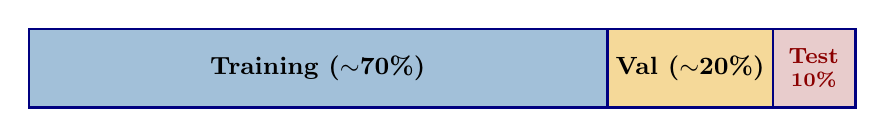
\begin{tikzpicture}
    % Full bar
    \fill[softblue!30] (0,0) rectangle (10.5,1);
    % Train
    \fill[softblue!50] (0,0) rectangle (7.35,1);
    % Val
    \fill[softorange!40] (7.35,0) rectangle (9.45,1);
    % Test
    \fill[darkred!20] (9.45,0) rectangle (10.5,1);
    % Borders
    \draw[uzhblue, thick] (0,0) rectangle (10.5,1);
    \draw[uzhblue, thick] (7.35,0) -- (7.35,1);
    \draw[uzhblue, thick] (9.45,0) -- (9.45,1);
    % Labels
    \node[font=\small\bfseries] at (3.67,0.5) {Training ($\sim$70\%)};
    \node[font=\small\bfseries] at (8.4,0.5) {Val ($\sim$20\%)};
    \node[font=\footnotesize\bfseries, darkred, align=center] at (9.97,0.5) {Test\\[-1pt]{\scriptsize 10\%}};
\end{tikzpicture}
\end{center}

\vspace{0.4cm}
\begin{columns}[T]
\column{0.32\textwidth}
\begin{block}{\centering Training set}
    \centering
    {\small Used to fit model parameters $\bm{\theta}$ via optimization.}
\end{block}

\column{0.32\textwidth}
\begin{block}{\centering Validation set}
    \centering
    {\small Used for model selection: hyperparameters, architecture, early stopping.}
\end{block}

\column{0.32\textwidth}
\begin{block}{\centering Test set}
    \centering
    {\small Touched \textbf{once} at the very end to report final performance.}
\end{block}
\end{columns}

\vspace{0.3cm}
\begin{alertblock}{Golden rule}
\centering Never use the test set for any decision during model development.
\end{alertblock}
\end{frame}

% --- Slide 49: Early Stopping ---
\begin{frame}{Early Stopping}
\begin{columns}[T]
\column{0.48\textwidth}
\begin{center}
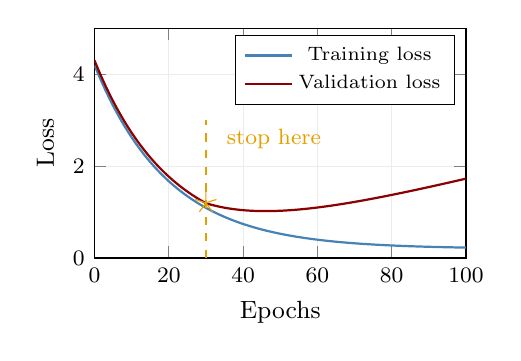
\begin{tikzpicture}
\begin{axis}[
    width=6.3cm, height=4.5cm,
    xlabel={Epochs}, ylabel={Loss},
    xmin=0, xmax=100, ymin=0, ymax=5,
    grid=major, grid style={gray!15},
    legend pos=north east,
    legend style={font=\scriptsize},
]
    % Training loss
    \addplot[thick, softblue, domain=0:100, samples=100]{4*exp(-0.05*x)+0.2};
    \addlegendentry{Training loss}
    % Validation loss
    \addplot[thick, darkred, domain=0:100, samples=100]{
        4*exp(-0.05*x) + 0.3 + 0.02*(x-30)*(x>30)
    };
    \addlegendentry{Validation loss}
    % Optimal point
    \draw[softorange, thick, dashed] (axis cs:30,0) -- (axis cs:30,3);
    \node[font=\footnotesize, softorange, anchor=west] at (axis cs:33,2.6) {stop here};
    \addplot[only marks, mark=star, mark size=4pt, softorange] coordinates {(30,1.2)};
\end{axis}
\end{tikzpicture}
\end{center}

\column{0.48\textwidth}
\textbf{Idea:} monitor the validation loss; stop when it starts rising.

\vspace{0.15cm}
\textbf{In practice:}
\begin{enumerate}\itemsep2pt
    \item Evaluate the validation loss after each epoch.
    \item Save the weights whenever it improves.
    \item Stop after $p$ epochs without improvement (``patience''); return the saved best weights.
\end{enumerate}

\vspace{0.2cm}
{\footnotesize It is the simplest effective regularizer, and it is essentially free.  Other standard options: an \textbf{$L_2$ penalty}, \textbf{dropout}, \textbf{data augmentation}.}
\end{columns}
\end{frame}

% --- Slide 50: L2 and Dropout ---
\begin{frame}{Regularization: The $L_2$ Penalty}
\begin{columns}[T]
\column{0.52\textwidth}
Add a penalty on the size of the weights (usually excluding biases):
\[
    \tilde{J}(\bm{\theta}) = J(\bm{\theta}) + \frac{\lambda}{2}\|\bm{\theta}\|_2^2
\]

\vspace{0.2cm}
Large weights are what let a network produce wild, wiggly functions.  Shrinking them biases the learner toward \emphc{smoother} hypotheses.

\vspace{0.2cm}
$\lambda$ is chosen on the \textbf{validation} set.

\column{0.44\textwidth}
\begin{alertblock}{$L_2 \neq$ weight decay under Adam}
\small For plain SGD the two are equivalent.  For \textbf{Adam} they are not, because the penalty gradient gets divided by $\sqrt{\hat{\bm{v}}_t}$ along with everything else.
\\[4pt]
Use \textbf{AdamW} if you want true decay (Loshchilov \& Hutter, 2019).
\end{alertblock}
\end{columns}
\end{frame}

% --- Dropout ---
\begin{frame}{Regularization: Dropout}
\begin{columns}[T]
\column{0.50\textwidth}
\textbf{Dropout} (Srivastava et al., 2014): during \emph{training}, independently zero each hidden unit with probability $p$ (typically $0.5$).

\vspace{0.3cm}
\begin{itemize}\itemsep4pt
    \item The network cannot rely on any single unit, so it must build \emphc{redundant} representations.
    \item At \emph{test} time all units are active, with no dropping.
    \item Equivalent to training an \textbf{ensemble} of sub-networks that share weights.
\end{itemize}

\column{0.46\textwidth}
\begin{center}
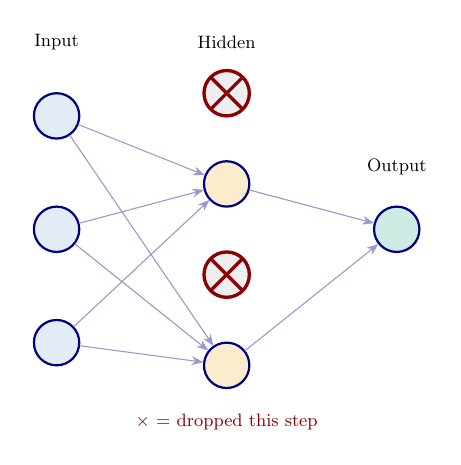
\begin{tikzpicture}[scale=0.72, transform shape,
    neuron/.style={circle, draw=uzhblue, thick, minimum size=8mm},
    dead/.style={circle, draw=darkred, very thick, minimum size=8mm, fill=uzhgreylight,
                 path picture={\draw[darkred,very thick] (path picture bounding box.south west)
                 -- (path picture bounding box.north east);
                 \draw[darkred,very thick] (path picture bounding box.north west)
                 -- (path picture bounding box.south east);}},
    arr/.style={-{Stealth[length=1.5mm]}, uzhblue!40}]

    \node[neuron, fill=softblue!15] (x1) at (0,2) {};
    \node[neuron, fill=softblue!15] (x2) at (0,0) {};
    \node[neuron, fill=softblue!15] (x3) at (0,-2) {};

    \node[dead] (h1) at (3,2.4) {};
    \node[neuron, fill=softorange!20] (h2) at (3,0.8) {};
    \node[dead] (h3) at (3,-0.8) {};
    \node[neuron, fill=softorange!20] (h4) at (3,-2.4) {};

    \node[neuron, fill=softgreen!20] (y) at (6,0) {};

    \foreach \i in {x1,x2,x3} {
        \draw[arr] (\i) -- (h2);
        \draw[arr] (\i) -- (h4);
    }
    \draw[arr] (h2) -- (y);
    \draw[arr] (h4) -- (y);

    \node[font=\small] at (0,3.3) {Input};
    \node[font=\small] at (3,3.3) {Hidden};
    \node[font=\small] at (6,1.1) {Output};
    \node[font=\small, darkred] at (3,-3.4) {$\times$ = dropped this step};
\end{tikzpicture}
\end{center}
\end{columns}
\end{frame}

% ============================================================================
% PART 6: OUTLOOK, SOFTWARE, AND EXERCISES
% ============================================================================

\section{Outlook and Practice}

% --- Section Divider ---
\begin{frame}{}
\begin{center}
{\Huge \textcolor{uzhblue}{Part V}}\\[0.8em]
{\LARGE Outlook, Software, and Exercises}
\end{center}
\end{frame}

% --- Slide 52: Beyond Feedforward Networks (outlook) ---
\begin{frame}{Beyond Feedforward Networks: Sequences and Attention}
Feedforward nets are \emph{memoryless}: $\hat{y}_t = f(\x_t)$.  For sequential data, three families add memory.

\vspace{0.3cm}
\begin{columns}[T]
\column{0.32\textwidth}
\begin{block}{RNN}
A hidden state $\bm{h}_t$ carries a running summary of the past.
\end{block}

\column{0.32\textwidth}
\begin{block}{LSTM / GRU}
Gates protect a memory lane, so signals survive many steps.
\end{block}

\column{0.32\textwidth}
\begin{block}{Transformer}
Attention lets every position read every other, in parallel.
\end{block}
\end{columns}

\vspace{0.35cm}
\begin{exampleblock}{Rule of thumb}
Specialized pattern, moderate history $\Rightarrow$ an LSTM is still a strong baseline.  Long context and parallelism matter $\Rightarrow$ start with a Transformer.
\end{exampleblock}

\end{frame}

% --- Slide 53: Software Ecosystem ---
\begin{frame}{Software Ecosystem}
\begin{center}

\begin{tikzpicture}[
    fw/.style={rectangle, draw=uzhblue, fill=uzhblue!8, rounded corners=5pt,
               minimum width=3.2cm, minimum height=1.8cm, align=center, font=\small}
]
    \node[fw, fill=softorange!15] (tf) at (0,0) {\textbf{\large TensorFlow}\\+ Keras\\{\scriptsize Google, 2015}};
    \node[fw, fill=darkred!8] (pt) at (5.2,0) {\textbf{\large PyTorch}\\{\scriptsize Meta AI, 2017}};
    \node[fw, fill=softgreen!10] (jax) at (10.4,0) {\textbf{\large JAX}\\{\scriptsize Google, 2018}};
\end{tikzpicture}
\end{center}

\vspace{0.5cm}
\begin{itemize}
    \item \href{https://keras.io}{\textbf{Keras}} is a high-level API that runs on top of TensorFlow, PyTorch, or JAX, so you write once and run anywhere.
    \item Documentation and tutorials for all three are linked from the course repository.
\end{itemize}

\vspace{0.4cm}
\begin{exampleblock}{This morning}
\centering We use \textbf{TensorFlow / Keras}.  A first network is about ten lines of code.
\end{exampleblock}
\end{frame}

% --- Slide 54: Hands-On ---
\begin{frame}{What Comes Next, and What to Run}
\small
\begin{block}{11:00 -- 12:30: Deep Equilibrium Nets (part II)}
\small
Everything from this lecture (networks, losses, SGD, regularization) comes together when we train a neural network to solve a dynamic stochastic model.
\end{block}

\vspace{0.15cm}
\textbf{Warm-up exercise} (notebook \texttt{01\_06}): approximate the Genz (1987) test functions with a neural network.
\begin{itemize}\itemsep2pt
    \item Train networks on 10, 50, 100, 500 random points from $[0,1]^d$ for $d\in\{2,5,10\}$.
    \item Vary the \textbf{depth} (1--5 hidden layers), the \textbf{activation} (tanh, ReLU, Swish), and the \textbf{optimizer} (SGD, Adam).
    \item Plot test error vs.\ the number of training points, and watch the \emphc{curse of dimensionality}.
\end{itemize}

\vspace{0.1cm}
{\footnotesize Notebooks \texttt{01\_01} to \texttt{01\_05} cover the rest: basic ML, gradient descent and SGD, double descent, a first deep network, and the same tasks in PyTorch.}

\vspace{0.1cm}
\begin{center}
{\footnotesize\textbf{Materials:}~\href{https://github.com/sischei/summer-school-AI-for-economics-and-finance-2026}{course GitHub repository}~~$\cdot$~~\textbf{Platform:}~\href{https://nuvolos.cloud}{nuvolos.cloud} (no local setup required)}
\end{center}
\end{frame}

% --- Slide 55: Questions ---
\begin{frame}{}
\begin{columns}[c]
\column{0.45\textwidth}
\begin{center}
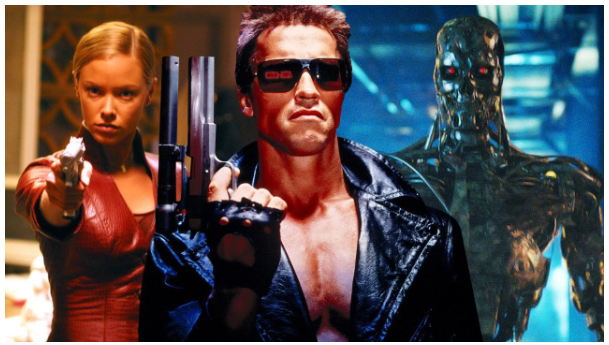
\includegraphics[width=0.85\textwidth]{figures/quest.png}
\end{center}

\column{0.50\textwidth}
\begin{center}
{\Huge \textcolor{uzhblue}{\textbf{Questions?}}}

\vspace{0.8cm}
{\large Simon Scheidegger}\\[4pt]
{\small HEC, University of Lausanne}\\[4pt]
\url{https://sischei.github.io}

\vspace{0.6cm}
{\small Materials:}\\[3pt]
{\footnotesize\href{https://github.com/sischei/summer-school-AI-for-economics-and-finance-2026}{github.com/sischei/summer-school-AI-for-economics-and-finance-2026}}
\end{center}
\end{columns}
\end{frame}


% ============================================================================
% APPENDIX (backup slides, shown only if time permits / on request)
% ============================================================================

\appendix

\begin{frame}{}
\vfill
\begin{center}
{\Huge \textcolor{uzhblue}{Backup slides}}
\end{center}
\vfill
\end{frame}

% --- Slide 12: Useful Materials ---
\begin{frame}{Useful Materials}
\begin{columns}[T]
\column{0.40\textwidth}
\begin{center}
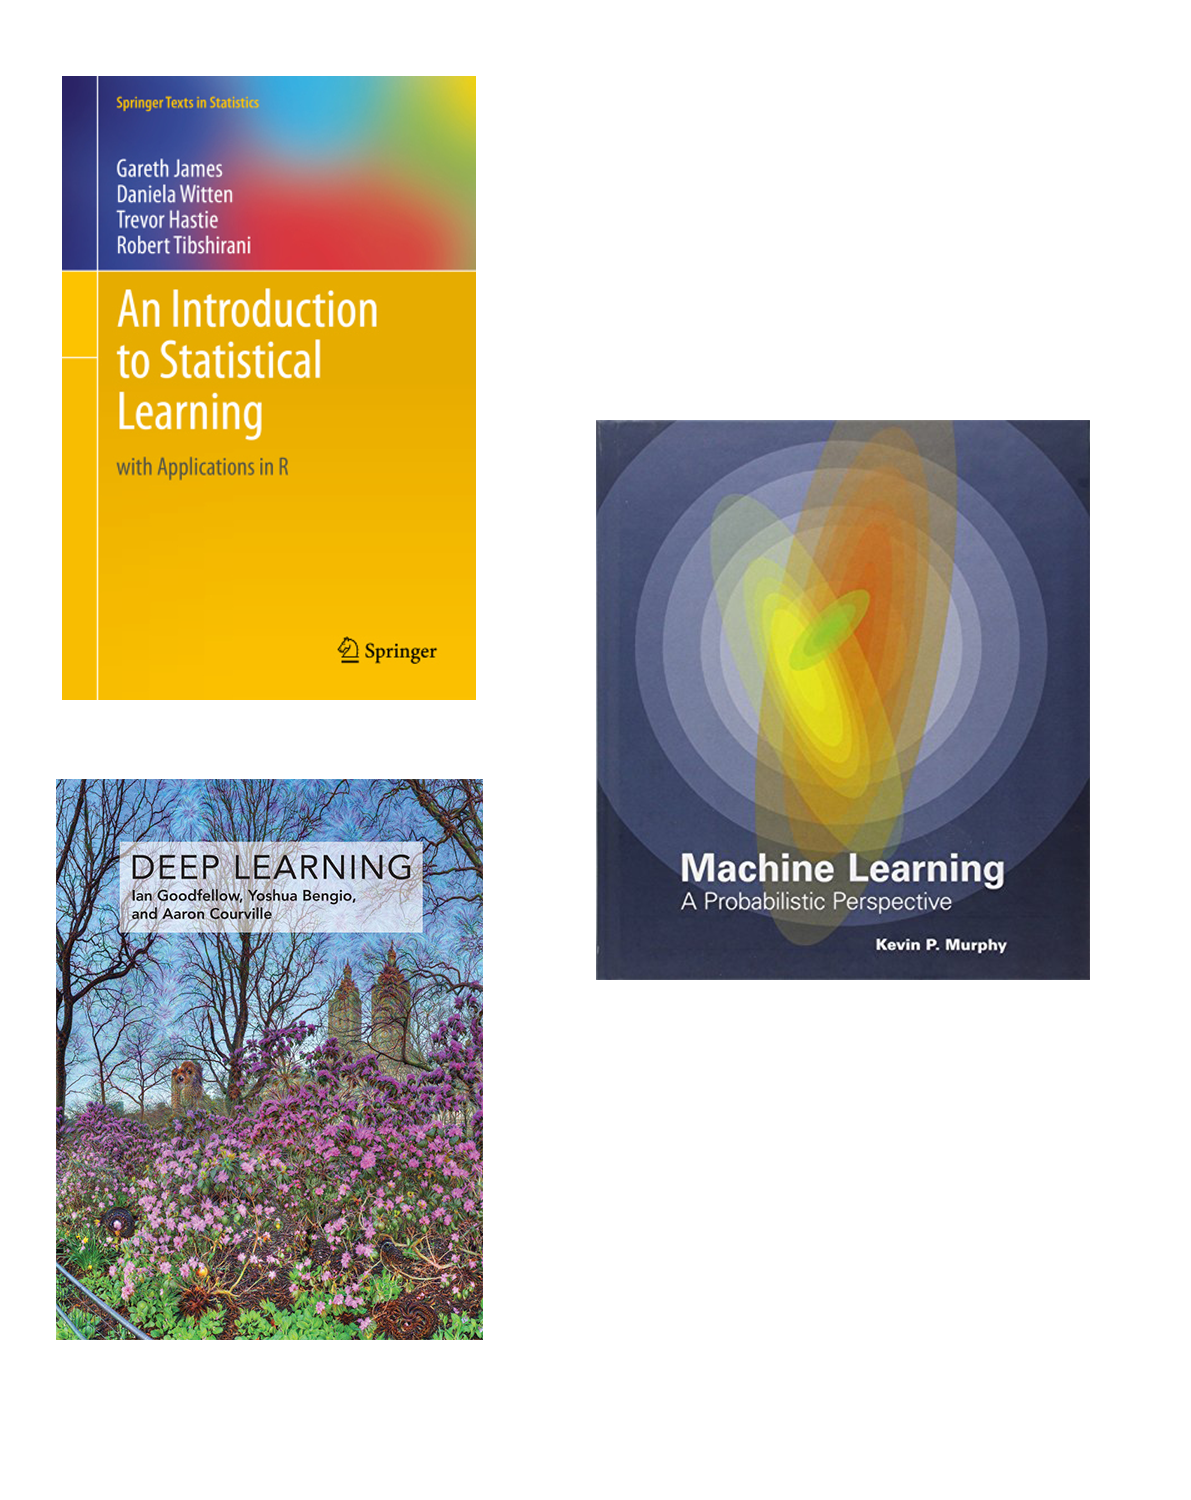
\includegraphics[width=0.85\textwidth]{figures/books1.png}
\end{center}

\column{0.56\textwidth}
\begin{enumerate}\itemsep8pt
    \item \textbf{S.\ J.\ D.\ Prince} (2023).\\ \textit{Understanding Deep Learning}. MIT Press. \emphc{(free PDF)}
    \item \textbf{I.\ Goodfellow, Y.\ Bengio, A.\ Courville} (2016).\\ \textit{Deep Learning}. MIT Press. \emphc{(free online)}
    \item \textbf{K.\ P.\ Murphy} (2022).\\ \textit{Probabilistic Machine Learning: An Introduction}. MIT Press. \emphc{(free PDF)}
    \item \textbf{G.\ James et al.} (2021).\\ \textit{An Introduction to Statistical Learning}. Springer. \emphc{(free PDF)}
\end{enumerate}
\end{columns}

\end{frame}


% --- Slide 51: Deep Double Descent ---
\begin{frame}{Deep Double Descent}
\begin{columns}[T]
\column{0.52\textwidth}
\begin{center}
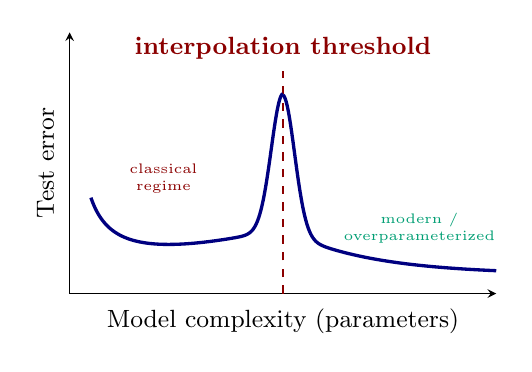
\begin{tikzpicture}
\begin{axis}[
    width=7cm, height=4.9cm,
    xlabel={Model complexity (parameters)},
    ylabel={Test error},
    xmin=0, xmax=10, ymin=0, ymax=6.8,
    grid=major, grid style={gray!15},
    xtick=\empty, ytick=\empty,
    axis lines=left,
    clip=false,
]
    % Interpolation threshold — vertical dashed marker + horizontal label above peak
    \draw[dashed, darkred, thick] (axis cs:5,0) -- (axis cs:5,5.8);
    \node[font=\small\bfseries, darkred, anchor=south]
        at (axis cs:5, 5.85) {interpolation threshold};

    % Classical regime + spike rise
    \addplot[very thick, uzhblue, domain=0.5:5, samples=200]
        {1.5/(x^0.7) + 0.15*(x^1.3) + 3.5*exp(-(x-5)^2/0.15)};
    % Modern regime + spike fall (identical spike term)
    \addplot[very thick, uzhblue, domain=5:10, samples=200]
        {0.5 + 1.17*exp(-0.5*(x-5)) + 3.5*exp(-(x-5)^2/0.15)};

    % Region labels
    \node[font=\tiny, darkred, align=center]
        at (axis cs:2.2, 3.0) {classical\\regime};
    \node[font=\tiny, softgreen, align=center]
        at (axis cs:8.2, 1.7) {modern /\\overparameterized};
\end{axis}
\end{tikzpicture}
\end{center}

\column{0.45\textwidth}
{\scriptsize The classical U turns into a \textbf{second descent} once the model is \emphc{overparameterized}. Three regimes along the curve:

\vspace{0.08cm}
\textcolor{darkred}{\textbf{1. Classical}} ($n_\text{par}\!<\!n_\text{data}$): the familiar bias--variance U: small models underfit, larger ones chase noise.

\vspace{0.06cm}
\textcolor{darkred}{\textbf{2. Interpolation peak}} ($n_\text{par}\!\approx\!n_\text{data}$): model \emph{just} fits the training set; among all zero-error solutions the optimizer's pick is unstable $\Rightarrow$ variance explodes.

\vspace{0.06cm}
\textcolor{softgreen}{\textbf{3. Modern}} ($n_\text{par}\!\gg\!n_\text{data}$): GD appears to select a low-complexity, \emphc{minimum-norm-like} interpolator, provable for linear/kernel models but conjectural for deep nets.

\vspace{0.06cm}
\emphc{Caveat:} the peak is often absent under proper regularization, and more \emph{data} can also hurt near the threshold (Nakkiran et al.\ 2019).

{\scriptsize Belkin et al.\ (2019); Nakkiran et al.\ (2019).}}
\end{columns}
\end{frame}


\end{document}
